\documentclass[a4paper,fleqn]{cas-sc}

\usepackage{amsmath,amssymb}
\usepackage{booktabs}
\usepackage{graphicx}
\usepackage{float}
\usepackage{placeins}
\usepackage{multirow}
\usepackage{siunitx}
\usepackage{array}
\usepackage{tabularx}
\usepackage{mdframed}
\usepackage{algorithm}
\usepackage{algpseudocode}
\usepackage{tikz}
\usetikzlibrary{arrows.meta,positioning,shapes.geometric,fit,calc,backgrounds,decorations.pathreplacing}
\graphicspath{{figures/}}
\setlength{\textfloatsep}{8pt plus 2pt minus 2pt}
\setlength{\floatsep}{8pt plus 2pt minus 2pt}
\setlength{\intextsep}{8pt plus 2pt minus 2pt}
\setlength{\abovecaptionskip}{4pt}
\setlength{\belowcaptionskip}{0pt}
\raggedbottom

\begin{document}
\let\WriteBookmarks\relax
\def\floatpagepagefraction{1}
\def\textpagefraction{.001}

\shorttitle{Feasible-support hybrid SAC for CAES plant dispatch}
\title[mode=title]{Plant-level weekly dispatch of a thermal--battery--CAES system with state-dependent multi-mode commands: a feasible-support hybrid soft actor--critic approach on a high-fidelity Modelica twin}

\begin{abstract}
Weekly price-taker dispatch of a thermal--battery--compressed-air (CAES) plant couples Shandong time-of-use (TOU) cash with a China National ETS carbon charge, spill/unserved penalties and battery wear. The CAES electric command lives in a disconnected device envelope that further shrinks with mode locks and inventory margins, so the admissible hybrid action is a \emph{state-dependent support} \(\mathcal{A}(s)\): admissible modes \(\mathcal{K}(s)\) and mode-conditioned magnitude intervals \(\mathcal{M}_k(s)\). Convex programmes typically relax that support; continuous DRL on a single box channel is a poor match to multi-mode plant commands. This paper states the plant on a MWORKS Sysplorer Modelica model exported as an FMI functional mock-up unit (FMU)---using FMI as an exchange standard for closed-loop verification, not as a claimed novelty---and proposes a \emph{feasible-support hybrid soft actor--critic} (FS-HSAC): a same-timescale hybrid policy that issues thermal load rate, battery power and a CAES pair $(\mathrm{mode},\mathrm{magnitude})$ with densities defined on \(\mathcal{M}_k(s)\), exact mode enumeration and dual temperatures. A residual feasibility classifier and an adopted GiveSafe shield handle residual twin constraints. Projected continuous SAC/TD3 and a fixed-band hybrid SAC remain ablations. Full-week economics are reported only after a shared results gate; the claim is support-consistent hybrid learning on the twin, not unconditional cash dominance over MILP or hierarchical RL.
\end{abstract}

\begin{highlights}
\item Sysplorer FMU thermal--battery--CAES plant under Shandong TOU and National ETS, with multi-mode CAES commands written as operating constraints rather than a ``discovery''.
\item State-dependent hybrid action support $\mathcal{A}(s)$: admissible modes $\mathcal{K}(s)$ and dynamic magnitude intervals $\mathcal{M}_k(s)$.
\item FS-HSAC: per-mode magnitude heads with Jacobian-corrected densities on $\mathcal{M}_k(s)$, exact mode enumeration, dual temperatures, residual feasibility learning and adopted GiveSafe.
\end{highlights}

\begin{keywords}
Multi-energy system \sep hybrid-action reinforcement learning \sep soft actor--critic \sep feasible action support \sep comprehensive cost \sep carbon pricing \sep time-of-use tariff \sep Modelica \sep FMU \sep CAES
\end{keywords}

\maketitle

% =====================================================================
% Nomenclature (framed two-column symbol table)
% =====================================================================
\begin{table}[H]
\centering
\small
\setlength{\tabcolsep}{4pt}
\renewcommand{\arraystretch}{1.1}
\begin{mdframed}[linewidth=0.7pt,linecolor=black,
  innerleftmargin=6pt,innerrightmargin=6pt,
  innertopmargin=4pt,innerbottommargin=4pt]
  \centering\textbf{Nomenclature}\par\medskip
  \begin{tabularx}{\linewidth}{@{}l X @{\quad} l X @{}}
    \toprule
    \multicolumn{4}{@{}l}{\textit{Indices and sets}} \\
    \midrule
    $t$ & hour index in a weekly episode, $t=0,\ldots,T-1$ ($T=168$) &
    $i$ & device / inventory index \\
    $\mathcal{S},\mathcal{A}(s)$ & state space and state-dependent hybrid action support &
    $\mathcal{K}(s),\mathcal{M}_k(s)$ & admissible CAES modes and magnitude interval for mode $k$ \\
    $\mathcal{F}(s)$ & dynamic feasible set used to build $\mathcal{A}(s)$ &
    $k_t,\,\mu_t$ & CAES mode and normalised magnitude \\
    \midrule
    \multicolumn{4}{@{}l}{\textit{Plant and market variables}} \\
    \midrule
    $P_t^{\mathrm{th/bat/caes}}$ & thermal / battery / CAES electric power &
    $P_t^{\mathrm{w/pv}},P_t^{\mathrm{load/grid}}$ & wind / PV / load / grid power \\
    $P_t^{\mathrm{curt}},P_t^{\mathrm{uns}}$ & curtailment and unserved power &
    $G_t,v_t,T_t^{\mathrm{air}}$ & irradiance, wind speed, ambient temperature \\
    $s_{t,\mathrm{bat/gas}}$ & battery and CAES gas SoC &
    $s_{t,\mathrm{hot/cold}}$ & CAES hot/cold thermal inventories \\
    $p_t,T_t^{\mathrm{gas}}$ & CAES gas pressure and temperature &
    $\eta,E_{\mathrm{cap}},p_{\mathrm{norm}}$ & battery efficiency, energy capacity, gas rating \\
    $\lambda_t^{\mathrm{buy/sell}}$ & TOU purchase / sale prices &
    $E_t^{\mathrm{buy/sell}}$ & grid purchase / sale energy \\
    $\Delta J_t^{\mathrm{cash}},J^{\mathrm{cash}}$ & cash-flow increment and weekly cash objective &
    $\Delta m_t,\pi_{\mathrm{CO_2}},J^{\mathrm{gen}}$ & CO$_2$ mass, ETS price, comprehensive objective \\
    $C_t^{CUT},C_t^{\mathrm{deg}}$ & curtailment/unserved cost, battery cycle cost &
    $C_t^{\mathrm{su}},C_t^{\mathrm{grid}}$ & CAES startup cost, soft interchange-contract cost \\
    $C_t^{\mathrm{op}}$ & device O\&M / fuel cash cost &
    $CC$ & comprehensive cost $CC=-J^{\mathrm{gen}}$ (primary ranking) \\
    $u_{\mathrm{tp}},u_{\mathrm{bat}},u_{\mathrm{caes}}$ & thermal / battery / CAES dispatch commands &
    --- & --- \\
    \midrule
    \multicolumn{4}{@{}l}{\textit{Feasible-support hybrid SAC}} \\
    \midrule
    $s_t,\,a_t$ & MDP state and physical FMU action &
    $m_t\in\{0,1\}^3$ & one-hot CAES mode (discharge / idle / charge) \\
    $M(s)$ & Boolean mode mask from $\mathcal{K}(s)$ &
    $\pi_{\theta}=\pi_d\pi_c$ & hybrid actor (discrete $\times$ continuous on $\mathcal{M}_k$) \\
    $\alpha_d,\alpha_c$ & discrete / continuous entropy temperatures &
    $C_{\psi}$ & residual twin feasibility classifier \\
    $r^{\mathrm{ext}}$ & extrinsic plant reward from $J^{\mathrm{gen}}$ &
    $\Pi_{\mathcal{F}}$ & GiveSafe acceptance onto $\mathcal{F}(s)$ \\
    $\gamma$ & discount factor &
    $\mathcal{D}_{\mathrm{B}},\mathcal{D}_{\mathrm{F}}$ & Bellman replay / feasibility replay \\
    \midrule
    \multicolumn{4}{@{}l}{\textit{Abbreviations}} \\
    \midrule
    FS-HSAC & feasible-support hybrid soft actor--critic &
    SAC & soft actor--critic (ablations: projected / fixed-band) \\
    TD3 & twin delayed DDPG (projected / hybrid ablation) \\
    PSO & particle swarm optimisation &
    TOU & time-of-use \\
    CAES & compressed-air energy storage &
    FMU & functional mock-up unit (FMI) \\
    ETS & emissions trading scheme &
    GHTD3 & goal-conditioned hierarchical TD3 (related) \\
    \bottomrule
  \end{tabularx}
\end{mdframed}
\end{table}
\FloatBarrier

% =====================================================================
\section{Introduction}
\label{sec:introduction}
% =====================================================================

Deep decarbonisation and China's national carbon market couple electricity markets with abatement costs at multi-energy plants~\cite{zhou2023iesdrl,yang2024planning,icap2025chinaets}. Provincial time-of-use (TOU) tariffs create peak--valley incentives~\cite{ndrc2021tou,shandong2023tou}, while an emissions trading scheme (ETS) attaches a monetary charge to thermal output and grid imports. This paper studies \emph{plant-level price-taker operation} of a thermal--battery--CAES facility: maximise a \emph{comprehensive monetary objective}---weekly net cash flow net of ETS-priced carbon, curtailment/unserved penalties, battery cycle cost, CAES startup cost and a soft interchange-contract charge---with soft week-end inventory shaping rather than a hard SoC veto, and rather than ISO market clearing~\cite{emmanuel2020market,pei2024pricetaker}. Hybrid continuous--discrete actions, CAES mode locks and thermal ramps render unconstrained plant interaction operationally unsafe and computationally demanding.

Model-based programmes remain useful baselines but typically require convexification of CAES thermodynamics or face restrictive budgets on hybrid spaces~\cite{cui2025ghtd3}. Deep reinforcement learning (DRL)~\cite{sutton2018rl,fujimoto2018td3,haarnoja2018sac} learns closed-loop policies by interaction. In multi-energy DRL studies the training environment is often an algebraic or otherwise simplified plant model; closed-loop evaluation on an FMI-exported multi-physics Modelica model of multi-tank CAES thermo-gas coupling remains comparatively less common. Hierarchical goal-conditioned controllers such as GHTD3~\cite{cui2025ghtd3} and option-style OCTD3 address multi-timescale inventory as the method identity; option initiation sets can restrict when a mode may start, but they do not by themselves provide a same-hour maximum-entropy density over a small discrete mode set and its mode-conditioned magnitude intervals. On the present Sysplorer FMU the CAES command is disconnected and further restricted by state, so we ask whether the policy is defined on the state-dependent support
\begin{equation*}
\mathcal{A}(s)
=
\mathcal{A}_{\mathrm{tp}}(s)\times
\mathcal{A}_{\mathrm{bat}}(s)\times
\bigcup_{k\in\mathcal{K}(s)}
\bigl(\{k\}\times\mathcal{M}_k(s)\bigr),
\end{equation*}
where $\mathcal{K}(s)$ is the set of currently admissible modes and $\mathcal{M}_k(s)$ the allowable magnitude interval for mode~$k$~\cite{garcia2015safe,sun2024constrained}. We therefore develop a \emph{feasible-support hybrid soft actor--critic} (FS-HSAC): a same-timescale hybrid policy with a discrete mode head and continuous magnitude heads on $\mathcal{M}_k(s)$. GiveSafe is used as the final execution screen, not as a claimed algorithmic novelty.

Three gaps remain. (1)~\textbf{Model and verification scope.} Weekly thermal--battery--CAES operation under Shandong TOU and National ETS pricing, with device envelope $u_{\mathrm{caes}}\in[-1,-0.33]\cup\{0\}\cup[0.86,1]$, mode locks and inventory margins, verified in closed loop on an FMI-exported Sysplorer twin (FMI as exchange standard). (2)~\textbf{State-dependent hybrid support.} The scheduling object requires a unified support $\mathcal{A}(s)$ with $\mathcal{K}(s)$ and $\mathcal{M}_k(s)$ written into the policy density, beyond box continuous actions or inventory-goal hierarchies alone. (3)~\textbf{Same-timescale hybrid solver.} With three modes decided jointly with magnitudes every hour, a maximum-entropy hybrid SAC that enumerates modes exactly is a direct design; we do not claim that hierarchical RL cannot address the same plant.

Table~\ref{tab:lit} positions related work.

\begin{table}[!htbp]
\centering
\caption{Comparison of related scheduling studies (selected).}
\label{tab:lit}
\scriptsize
\begin{tabular}{@{}p{2.0cm}cccccp{1.6cm}@{}}
\toprule
Study & Hybrid act. & Safety & High-fid.\ twin & State supp. & Market & Method \\
\midrule
Zhou et al.~\cite{zhou2023iesdrl} & -- & -- & -- & -- & tariff / cost & flat DRL \\
Sun et al.~\cite{sun2024constrained} & -- & $\checkmark$ & -- & -- & multi-energy & constr.\ RL \\
Cui et al.~\cite{cui2025ghtd3} & -- & -- & -- & -- & TOU / cost & GHTD3 \\
Pei et al.~\cite{pei2024pricetaker} & -- & -- & -- & -- & spot PT & optimisation \\
\textbf{This work} & $\checkmark$ & $\checkmark$ (adopt) & $\checkmark$ (FMU) & $\checkmark$ & TOU PT + ETS & FS-HSAC \\
\bottomrule
\end{tabular}
\end{table}

The contributions follow object $\rightarrow$ formalisation $\rightarrow$ solver $\rightarrow$ verification.
\begin{enumerate}
\item \textbf{Object (C1).} A thermal--battery--CAES Sysplorer Modelica plant with multi-mode CAES commands~\eqref{eq:caes-legal}, mode locks and gas--thermal DAE dynamics, exported as an FMI FMU for closed-loop interaction. Weekly $J^{\mathrm{gen}}$ couples TOU cash, ETS carbon, spill/unserved energy and battery wear; week-end inventory enters only as a soft terminal bonus in~$r^{\mathrm{ext}}$.
\item \textbf{Formalisation (C2).} Dispatch is cast as a hybrid MDP with state-dependent support $\mathcal{A}(s)$ built from admissible modes $\mathcal{K}(s)$ and mode-conditioned intervals $\mathcal{M}_k(s)$, so that the policy density is defined on the same support the twin can accept.
\item \textbf{FS-HSAC solver (C3).} A same-timescale hybrid SAC with per-mode magnitude heads and Jacobian-corrected maps onto $\mathcal{M}_k(s)$, exact mode enumeration, dual temperatures $\alpha_d/\alpha_c$, a hybrid critic on $(u_{\mathrm{tp}},u_{\mathrm{bat}},\mathrm{onehot}(k),\mu)$, and a residual feasibility classifier $C_{\psi}$. GiveSafe is adopted; projected continuous SAC/TD3 and fixed-band hybrid SAC are ablations (Section~\ref{sec:ablation}). We do not claim superiority over multi-timescale HRL as a general principle.
\item \textbf{Verification (C4).} A fair weekly protocol across winter / transition / summer windows, with cost-component tables and sensitivity on carbon price and feasibility-margin scaling once the shared results gate passes.
\end{enumerate}

Section~\ref{sec:system} describes the plant and TOU setting. Section~\ref{sec:problem} formulates physics, the comprehensive objective and the state-dependent hybrid MDP. Section~\ref{sec:method} presents FS-HSAC. Section~\ref{sec:setup} states the fair weekly protocol. Section~\ref{sec:results} reports economics after the results gate. Section~\ref{sec:conclusion} concludes.

% =====================================================================
\section{System description}
\label{sec:system}
% =====================================================================

\subsection{Plant topology and modelling workflow}

Figure~\ref{fig:topology} summarises the multi-energy plant. The supply layer comprises wind, photovoltaic (PV) generation and a grid interface under TOU buy/sell prices. The conversion layer centres on a thermal unit commanded by a continuous load rate $u_{\mathrm{tp}}$ and a CAES train commanded by discrete mode and continuous magnitude. The storage layer comprises a battery with continuous power command $u_{\mathrm{bat}}$ and CAES gas and thermal inventories (gas tank, hot and cold tanks). The demand layer balances electric load and grid exchange.

Plant dynamics follow first-principles multi-physics: thermal ramping and fuel use; electrochemical battery SoC with round-trip efficiency; multi-tank CAES gas storage with thermo-mechanical coupling and mode locks; renewable availability; and nodal power balance with curtailment and unserved residual. The complete Modelica model is constructed and parameterised in \textbf{MWORKS Sysplorer}, then exported as an FMI-compliant FMU. Closed-loop optimisers and learning agents interact with this FMU at a communication interval of one hour, reading plant states and writing hybrid set-points. Exogenous TOU prices and resource profiles provide market and boundary conditions without replacing the internal differential--algebraic dynamics.

\begin{figure}[!htbp]
\centering
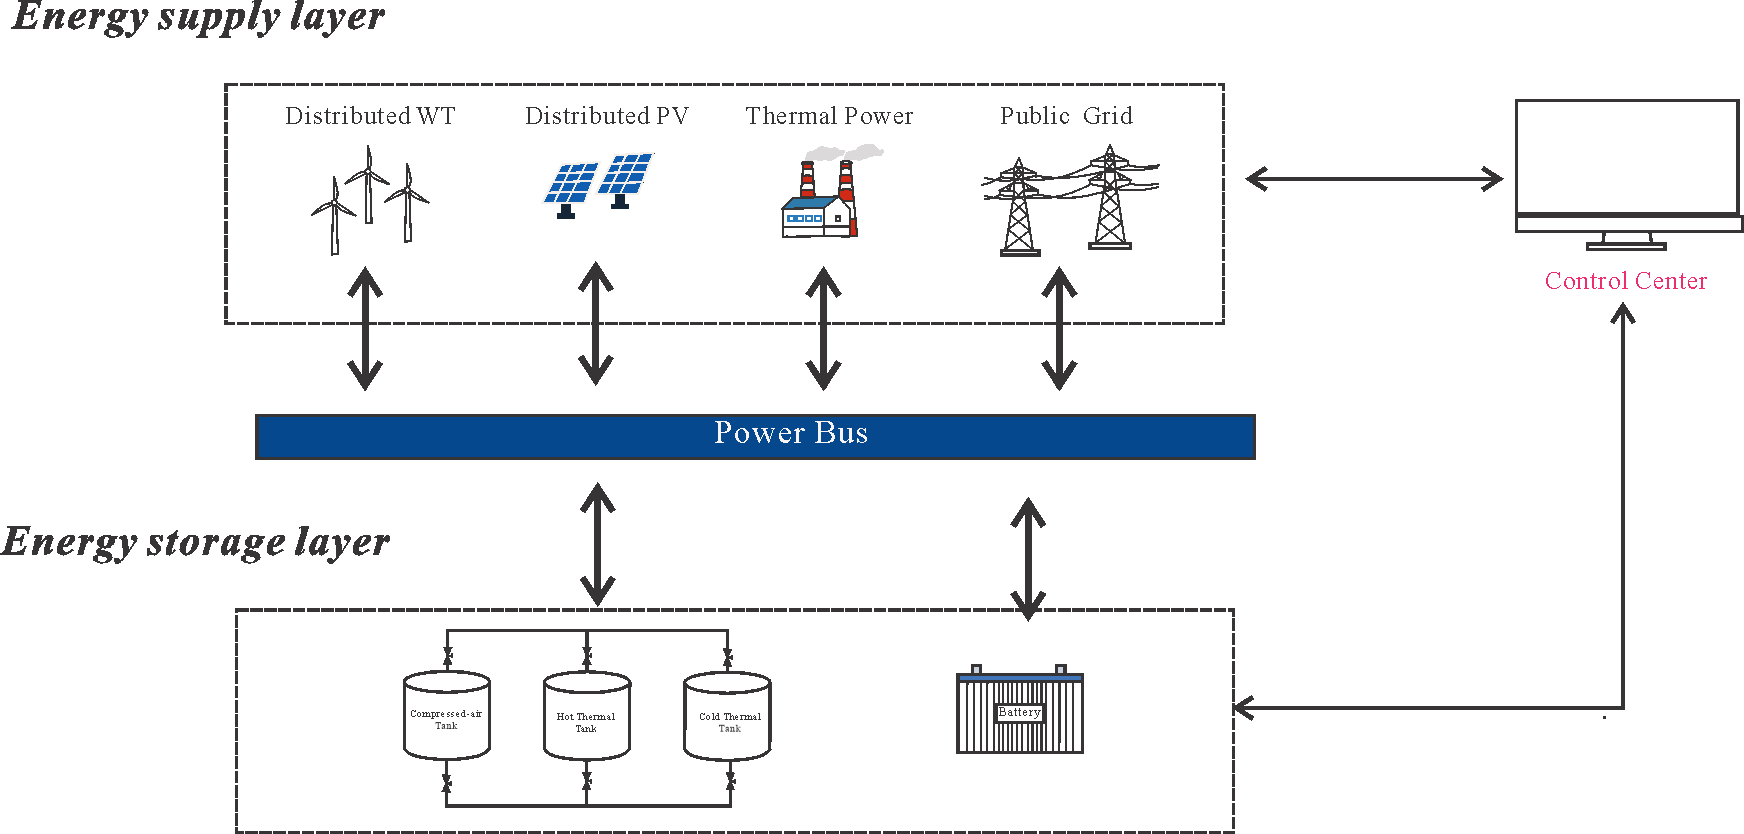
\includegraphics[width=\textwidth]{fig_topology}
\caption{Topology of the thermal--battery--CAES multi-energy plant. Device and network physics are modelled in MWORKS Sysplorer (Modelica) and exported as an FMI FMU for closed-loop dispatch.}
\label{fig:topology}
\end{figure}
\FloatBarrier

\subsection{Price-taker TOU market}

The plant is a price-taker under a \emph{constructive} Shandong industrial/commercial TOU delivered-price path whose band windows and float ratios follow provincial TOU policy and the 2026 State Grid Shandong announcement, while absolute yuan/kWh levels are assembled from an illustrative proxy-purchase base plus the fourth-cycle 110~kV T\&D energy charge~\cite{ndrc2021tou,shandong2023tou,shandong2026tou,ndrc2023td}. Absolute buy levels are \emph{not} claimed as a monthly agency settlement schedule. The flat sell price is illustrative. Figure~\ref{fig:price} shows a sample winter day; Fig.~\ref{fig:boundary} shows weekly wind, irradiance, load and TOU profiles for winter, transition and summer windows used in the case study. Table~\ref{tab:params} lists plant ratings, legal CAES bands and the market operating points used throughout.

\begin{table}[!htbp]
\centering
\caption{Plant and market parameters used in the weekly case study.}
\label{tab:params}
\scriptsize
\begin{tabular}{@{}lll@{}}
\toprule
Quantity & Value & Note \\
\midrule
Wind / PV nameplate & 300 / 260~MW & Resource-limited injection \\
Thermal \(P_{\min}\)--\(P_{\mathrm{cap}}\) & 50--150~MW & Load rate \(u_{\mathrm{tp}}\in[1/3,1]\); no shut-down \\
Battery power / energy & 100~MW / 500~MWh & \(\eta=0.85\) on discharge \\
CAES electric rating & 150~MW & Legal \(u_{\mathrm{caes}}\in[-1,-0.33]\cup\{0\}\cup[0.86,1]\) \\
Grid hard / contract limits & \(\pm500\) / \(\pm200\)~MW & Soft contract priced in \(J^{\mathrm{gen}}\) \\
TOU buy (S/P/F/V/D) & 1.136 / 0.986 / 0.635 / 0.284 / 0.183~CNY/kWh & Constructive Shandong mechanism path \\
TOU sell & 0.1875~CNY/kWh & Illustrative flat export price \\
ETS price \(\pi_{\mathrm{CO_2}}\) & 97.49~CNY/tCO\(_2\) & 2024 YE national CEA close~\cite{mee2025etsnews,mee2025etsreport} \\
Thermal EF / grid EF / benchmark \(\beta\) & 0.85 / 0.6191 / 0.8049~t/MWh & Scenario EF; Shandong 2023 EF; Class~II 2024 \(\beta\)~\cite{mee2023ef,mee2024quota} \\
Curtailment / unserved & 300 / 1000~CNY/MWh & Objective penalties; \(\approx\)GHTD3 \(\nu_{\mathrm{res}}\)~\cite{cui2025ghtd3} \\
CAES startup (scaled) & \(\approx 4617\)~CNY/event & Cui 2024 \(3.42\)~USD@800~kW + linear \(P\) extrapolation~\cite{cui2024caesbess} \\
Grid-contract excess & 600~CNY/MWh beyond \(\pm200\)~MW & Scenario soft band (not statutory) \\
Episode length \(T\) & 168~h & Weekly MDP; calendar only rotates week starts \\
\bottomrule
\end{tabular}
\end{table}

\begin{figure}[!htbp]
\centering
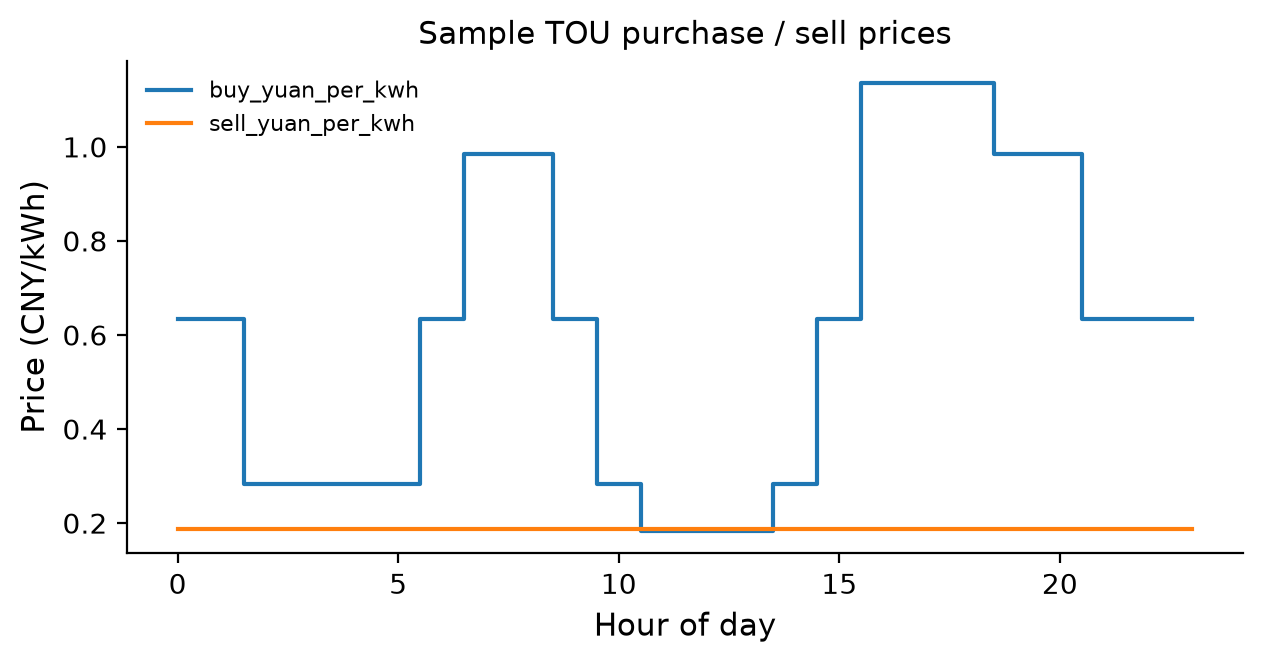
\includegraphics[width=0.68\textwidth]{fig_price_tou}
\caption{Constructive Shandong TOU purchase price on a sample winter day (mechanism-official bands; absolute levels assembled, not a monthly agency settlement schedule).}
\label{fig:price}
\end{figure}

\begin{figure}[!htbp]
\centering
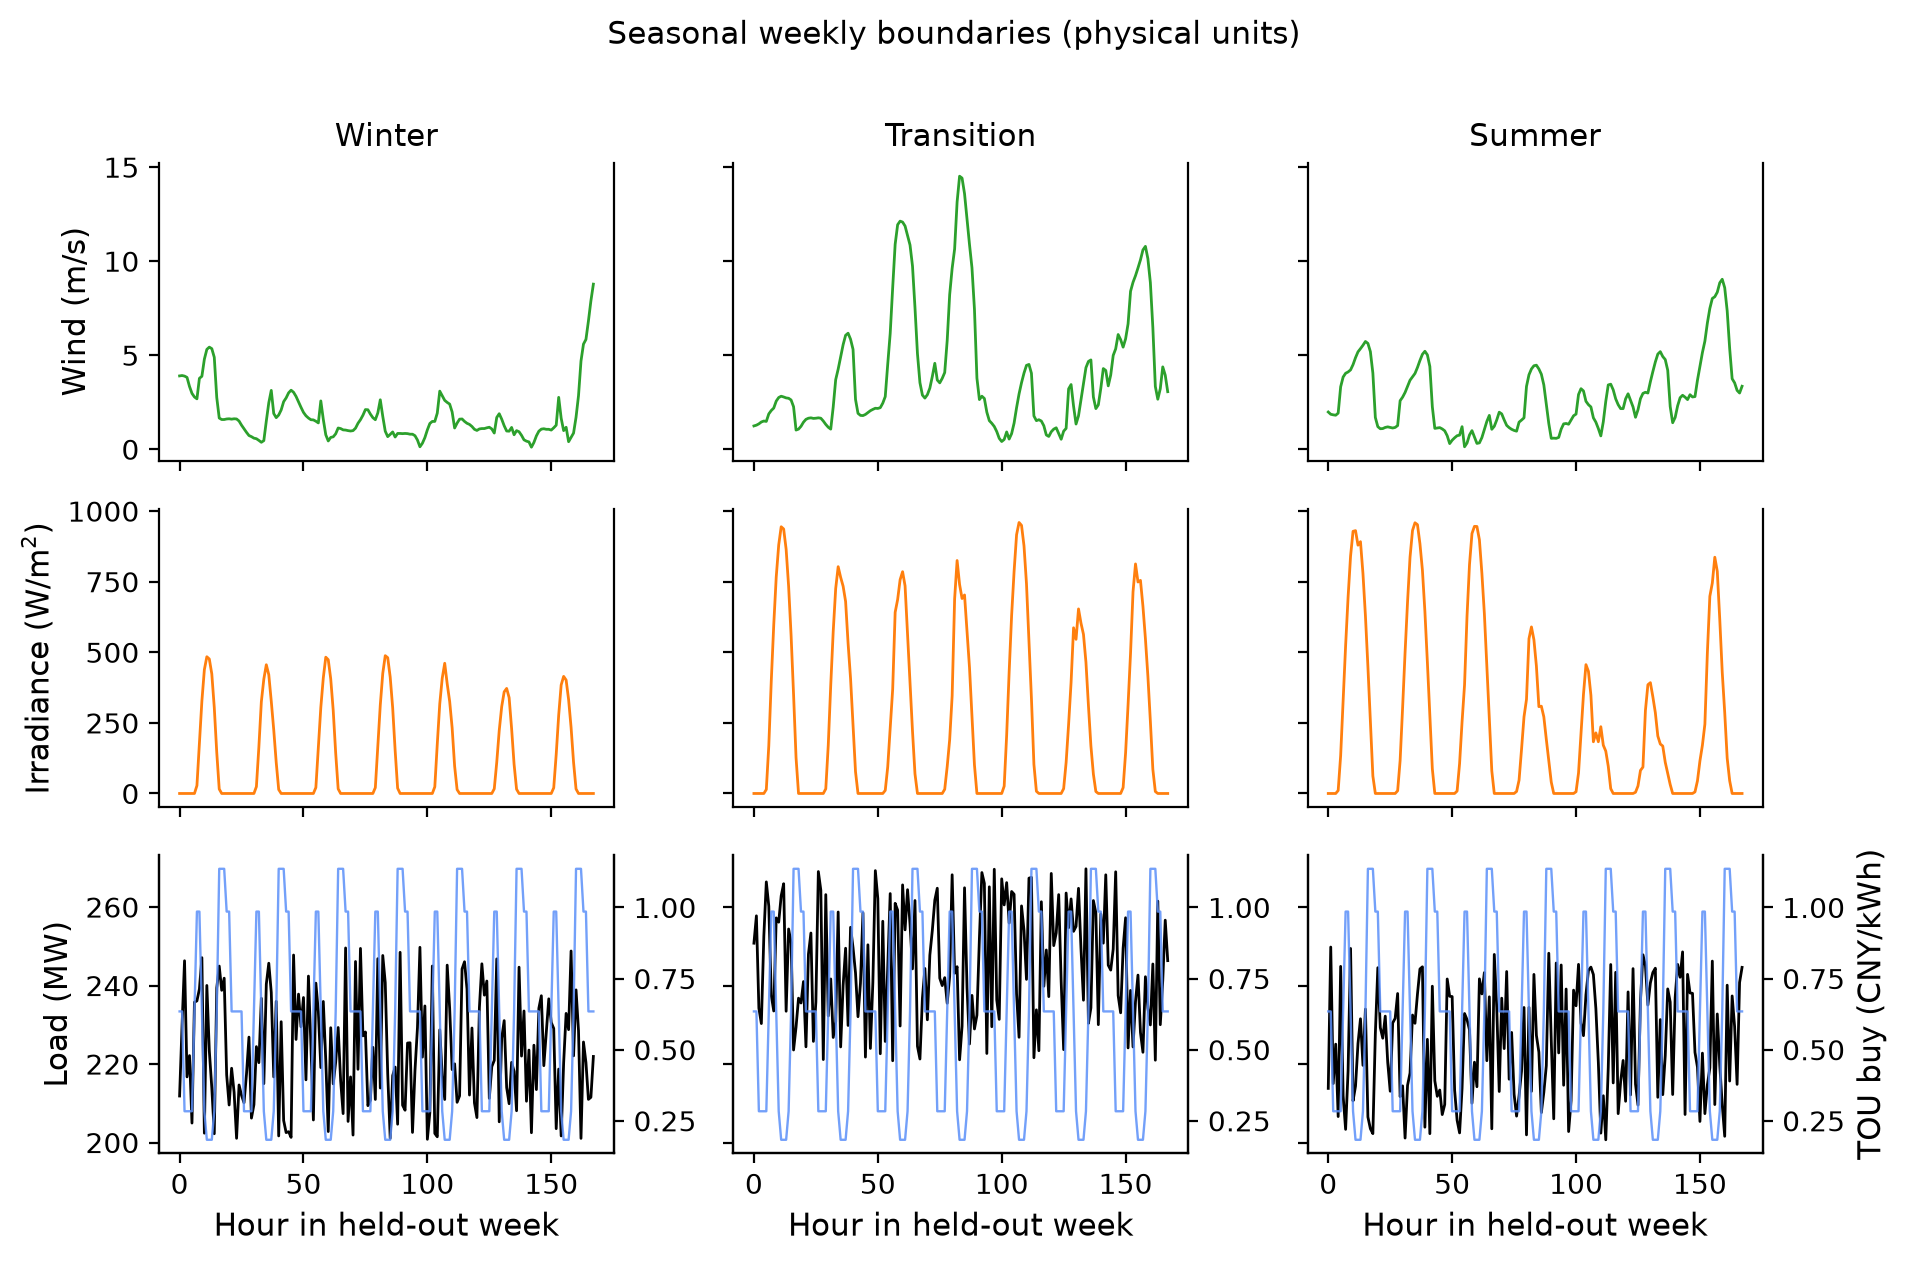
\includegraphics[width=\textwidth]{fig_seasonal_boundary}
\caption{Weekly wind speed, solar irradiance, electric load and TOU purchase price on the three held-out evaluation windows (physical units; irradiance is W/m$^2$, not normalised).}
\label{fig:boundary}
\end{figure}
\FloatBarrier

% =====================================================================
\section{Problem formulation}
\label{sec:problem}
% =====================================================================

This section formulates the multi-energy plant physics, operating constraints and market objective that define the \emph{weekly} scheduling problem (\(T=168\)~h). Continuous-time differential--algebraic equations of the plant (thermal unit, battery, multi-tank CAES, renewables and grid interface) are integrated in the Sysplorer-exported FMU with communication interval $\tau_s=1$~h; the relations below are the dispatch-level models realised by that twin and used by optimisers and learning agents. The 8760~h plant calendar only rotates weekly episode starts; it is not an annual MDP. We adopt the following sign convention throughout: renewable and thermal generation are non-negative when injecting power; battery and CAES charge is positive and discharge is negative; grid import is positive. Component sets are
\begin{equation}
\begin{aligned}
I_1&=\{\mathrm{w},\mathrm{pv}\},\quad
I_2=\{\mathrm{th},\mathrm{caes}\},\quad
I_3=\{\mathrm{bat},\mathrm{gas},\mathrm{hot},\mathrm{cold}\},\\
I&=I_1\cup I_2\cup I_3.
\end{aligned}
\label{eq:sets}
\end{equation}

\subsection{Energy generation units}

\subsubsection{Photovoltaics}

PV available power depends on plane-of-array irradiance $G_t$, module surface temperature $T_t^{\mathrm{pv}}$ and nameplate capacity $P_n^{\mathrm{pv}}=260$~MW. With standard irradiance $G_{\mathrm{stc}}=1000$~W/m$^2$, standard temperature $T_{\mathrm{stc}}=298.15$~K, temperature coefficient $K_T=0.005$~K$^{-1}$ and conversion efficiency $\eta^{\mathrm{pv}}=0.95$,
\begin{equation}
P_t^{\mathrm{pv,avail}}
=
\max\Bigl(
P_n^{\mathrm{pv}}
\frac{G_t}{G_{\mathrm{stc}}}
\bigl[1-K_T\bigl(T_t^{\mathrm{pv}}-T_{\mathrm{stc}}\bigr)\bigr]
\eta^{\mathrm{pv}},\,0\Bigr).
\label{eq:pv}
\end{equation}
Module temperature is obtained from ambient temperature $T_t^{\mathrm{air}}$, wind speed $v_t$ and irradiance by the twin correlation
\begin{equation}
T_t^{\mathrm{pv}}
=
T_t^{\mathrm{air}}
+
0.0138\bigl(1+0.031(T_t^{\mathrm{air}}-273.15)\bigr)
\bigl(1-0.042\,v_t\bigr)G_t.
\label{eq:pv-temp}
\end{equation}
Actual injected PV power after bus curtailment satisfies $0\le P_t^{\mathrm{pv}}\le P_t^{\mathrm{pv,avail}}$.

\subsubsection{Wind turbines}

Wind available power follows a cubic power curve with cut-in, rated and cut-out speeds $v_{\mathrm{ci}}=3$~m/s, $v_{\mathrm{r}}=10$~m/s and $v_{\mathrm{co}}=15$~m/s on capacity $P_n^{\mathrm{w}}=300$~MW:
\begin{equation}
P_t^{\mathrm{w,avail}}
=
\begin{cases}
0, & 0\le v_t < v_{\mathrm{ci}}\ \text{or}\ v_t\ge v_{\mathrm{co}},\\[2pt]
P_n^{\mathrm{w}}\,\dfrac{v_t^{3}-v_{\mathrm{ci}}^{3}}{v_{\mathrm{r}}^{3}-v_{\mathrm{ci}}^{3}},
& v_{\mathrm{ci}}\le v_t < v_{\mathrm{r}},\\[6pt]
P_n^{\mathrm{w}}, & v_{\mathrm{r}}\le v_t < v_{\mathrm{co}}.
\end{cases}
\label{eq:wt}
\end{equation}
Turbine pitch is not a free decision variable. Actual wind injection obeys $0\le P_t^{\mathrm{w}}\le P_t^{\mathrm{w,avail}}$.

\subsection{Energy conversion units}

\subsubsection{Thermal generation}

Thermal electric power is commanded by the continuous load rate $u_{\mathrm{tp},t}$:
\begin{equation}
P_t^{\mathrm{th}} = u_{\mathrm{tp},t}\, P_{\mathrm{cap}}^{\mathrm{th}},
\qquad
u_{\min}\le u_{\mathrm{tp},t}\le u_{\max},
\label{eq:th}
\end{equation}
with $P_{\mathrm{cap}}^{\mathrm{th}}=150$~MW, $P_{\min}^{\mathrm{th}}=50$~MW, $u_{\min}=P_{\min}^{\mathrm{th}}/P_{\mathrm{cap}}^{\mathrm{th}}=1/3$ and $u_{\max}=1$ (no shut-down). Inter-hour ramping is enforced on the actual thermal power,
\begin{equation}
\bigl|P_t^{\mathrm{th}}-P_{t-1}^{\mathrm{th}}\bigr|
\le
\Delta_{\mathrm{th}}^{\max}
=
r_{\max}\,P_{\mathrm{cap}}^{\mathrm{th}}\,\tau_s,
\label{eq:th-ramp}
\end{equation}
where $r_{\max}=0.0025/60$~s$^{-1}$ is the Modelica load-rate limit (equivalently $0.15$~p.u.\ per hour). Fuel and O\&M costs enter $C_t^{\mathrm{op}}$ in~\eqref{eq:dJ}.

\subsubsection{CAES conversion}

CAES is a hybrid conversion--storage plant. The hybrid command comprises a discrete mode and continuous magnitude
\begin{equation}
m_{\mathrm{caes},t}\in\{\mathrm{charge},\mathrm{idle},\mathrm{discharge}\},\qquad
\mu_{\mathrm{caes},t}\in[0,1],
\label{eq:caes-cmd}
\end{equation}
mapped to a signed electric power command on capacity $P_{\mathrm{cap}}^{\mathrm{caes}}=150$~MW,
\begin{equation}
P_t^{\mathrm{caes}}
=
\begin{cases}
+\mu_{\mathrm{caes},t}\,P_{\mathrm{cap}}^{\mathrm{caes}}, & m=\mathrm{charge},\\
0, & m=\mathrm{idle},\\
-\mu_{\mathrm{caes},t}\,P_{\mathrm{cap}}^{\mathrm{caes}}, & m=\mathrm{discharge},
\end{cases}
\label{eq:caes-p}
\end{equation}
or equivalently $P_t^{\mathrm{caes}}=u_{\mathrm{caes},t}P_{\mathrm{cap}}^{\mathrm{caes}}$ with the non-convex legal set
\begin{equation}
u_{\mathrm{caes},t}
\in
[-1,-0.33]\cup\{0\}\cup[0.86,1]
\label{eq:caes-legal}
\end{equation}
encoding minimum compressor/expander loading. Mode locks and minimum-run dwell constraints further restrict admissible transitions of $m_{\mathrm{caes}}$. Electric power is realised as planned ($P^{\mathrm{act}}=P^{\mathrm{plan}}$); mass-flow set-points of air and thermal fluid scale with $|P_t^{\mathrm{caes}}|$ and reverse direction between compression and expansion.

\subsection{Energy storage units}

\subsubsection{Battery}

Battery power is commanded by $u_{\mathrm{bat},t}\in[-1,1]$ on $P_{\mathrm{cap}}^{\mathrm{bat}}=100$~MW:
\begin{equation}
P_t^{\mathrm{bat}} = u_{\mathrm{bat},t}\, P_{\mathrm{cap}}^{\mathrm{bat}}.
\label{eq:bat-p}
\end{equation}
With energy capacity $E_{\mathrm{cap}}=500$~MWh and discharge efficiency $\eta=0.85$ (charge path lossless as in the twin), the SoC dynamics are
\begin{equation}
\frac{\mathrm{d}s_{\mathrm{bat}}}{\mathrm{d}t}
=
\begin{cases}
P^{\mathrm{bat}}/E_{\mathrm{cap}}, & P^{\mathrm{bat}}\ge 0,\\[2pt]
P^{\mathrm{bat}}/(E_{\mathrm{cap}}\,\eta), & P^{\mathrm{bat}}<0,
\end{cases}
\label{eq:bat-soc}
\end{equation}
or, in hourly form with $[x]_+=\max(x,0)$ and $[x]_-=\max(-x,0)$,
\begin{equation}
s_{t+1,\mathrm{bat}}
=
s_{t,\mathrm{bat}}
+
\tau_s\frac{[P_t^{\mathrm{bat}}]_+ - [P_t^{\mathrm{bat}}]_-/\eta}{E_{\mathrm{cap}}}.
\label{eq:bat-soc-d}
\end{equation}
Inventory bounds are $s_{\mathrm{bat}}\in[0.1,0.9]$.

\subsubsection{CAES inventories}

CAES energy is stored as compressed air and two thermal fluid tanks. Gas SoC is pressure-based with rating $p_{\mathrm{norm}}=100$~bar,
\begin{equation}
s_{t,\mathrm{gas}}
=
\frac{p_t}{p_{\mathrm{norm}}},
\qquad
\underline{s}_{\mathrm{gas}}\le s_{t,\mathrm{gas}}\le \overline{s}_{\mathrm{gas}},
\label{eq:gas-soc}
\end{equation}
with $(\underline{s}_{\mathrm{gas}},\overline{s}_{\mathrm{gas}})=(0.6,1.0)$. Fixed-volume gas-tank mass and energy balances (ideal-air medium) evolve pressure $p$ and specific enthalpy $h$ under port mass flows $\dot m_{\mathrm{a}},\dot m_{\mathrm{b}}$ and wall heat $q_{\mathrm{w}}$,
\begin{align}
V\bigl(\partial_p\rho\,\dot p+\partial_h\rho\,\dot h\bigr)
&=
\dot m_{\mathrm{a}}+\dot m_{\mathrm{b}},
\label{eq:gas-mass}\\
V\bigl(-\dot p+\partial_p\rho\,\dot p\,h+\partial_h\rho\,\dot h\,h+\rho\dot h\bigr)
&=
\dot m_{\mathrm{a}}h_{\mathrm{a}}^{\mathrm{in}}
+
\dot m_{\mathrm{b}}h_{\mathrm{b}}^{\mathrm{out}}
+
q_{\mathrm{w}},
\label{eq:gas-energy}
\end{align}
with $q_{\mathrm{w}}=\alpha_{\mathrm{w}}S(T_{\mathrm{w}}-T)$ and gas temperature $T=T(p,h)$ (clipped at $253$~K). Hot and cold tanks store water at fixed pressure with free surface area $A$ and total volume $V_0=1.5\times10^{4}$~m$^3$. Level-based inventories
\begin{equation}
s_{t,i}
=
\frac{\ell_{t,i}}{V_0/A},
\qquad
i\in\{\mathrm{hot},\mathrm{cold}\},
\label{eq:thermal-soc}
\end{equation}
obey mass and enthalpy balances when within $(\underline{s}_i,\overline{s}_i)=(0.05,0.95)$,
\begin{equation}
\dot m_i=\dot m_{\mathrm{a},i}+\dot m_{\mathrm{b},i},\qquad
m_i\dot h_i
=
\dot m_{\mathrm{a},i}h_{\mathrm{a},i}^{\mathrm{in}}
+
\dot m_{\mathrm{b},i}h_{\mathrm{b},i}^{\mathrm{out}}+Q_{\mathrm{gen},i}.
\label{eq:tank-bal}
\end{equation}
Compression ($P^{\mathrm{caes}}>0$) charges the gas inventory and drives the thermal circuit one way; expansion ($P^{\mathrm{caes}}<0$) reverses the flows. Primary weekly recovery inventories are $s_{\mathrm{bat}}$ and $s_{\mathrm{gas}}$; hot/cold SoCs and temperatures $(T^{\mathrm{hot}},T^{\mathrm{cold}})$ are process states used in soft shaping. All inventories obey~\eqref{eq:socbox}.

\subsection{System operation constraints}

The electric bus closes the power balance with curtailment and unserved load. Let $P_t^{\mathrm{w,avail}},P_t^{\mathrm{pv,avail}}$ be renewable availability and $P_t^{\mathrm{load,plan}}$ the scheduled demand. Residual power after dispatchable assets is absorbed first by curtailing wind, then PV; residual deficit is met by demand response down to $20\%$ of plan, with remainder counted as unserved:
\begin{equation}
\begin{aligned}
&P_t^{\mathrm{th}}+P_t^{\mathrm{bat}}+P_t^{\mathrm{caes}}
+P_t^{\mathrm{w}}+P_t^{\mathrm{pv}}+P_t^{\mathrm{grid}}
=
P_t^{\mathrm{load}},\\
&0\le P_t^{\mathrm{w}}\le P_t^{\mathrm{w,avail}},\quad
0\le P_t^{\mathrm{pv}}\le P_t^{\mathrm{pv,avail}},\\
&P_t^{\mathrm{curt}}\ge 0,\quad
P_t^{\mathrm{uns}}\ge 0,\quad
0.2\,P_t^{\mathrm{load,plan}}\le P_t^{\mathrm{load}}\le P_t^{\mathrm{load,plan}}.
\end{aligned}
\label{eq:balance}
\end{equation}
Here $P_t^{\mathrm{curt}}$ is residual surplus after wind-then-PV curtailment and $P_t^{\mathrm{uns}}$ is residual shortfall after load reduction. Box and ramp limits, inventory bounds and grid exchange limits are
\begin{equation}
\underline{P}_{i}\le P_t^{i}\le \overline{P}_{i},\qquad
\bigl|P_t^{i}-P_{t-1}^{i}\bigr|\le \Delta_i^{\max},
\quad i\in\{\mathrm{th},\mathrm{bat}\},
\label{eq:box}
\end{equation}
\begin{equation}
\underline{s}_{i}\le s_{t,i}\le \overline{s}_{i},\qquad i\in\{\mathrm{bat},\mathrm{gas},\mathrm{hot},\mathrm{cold}\},
\label{eq:socbox}
\end{equation}
\begin{equation}
P_{\mathrm{grid}}^{\min}\le P_t^{\mathrm{grid}}\le P_{\mathrm{grid}}^{\max},
\label{eq:grid}
\end{equation}
with $(P_{\mathrm{grid}}^{\min},P_{\mathrm{grid}}^{\max})=(-500,500)$~MW. Actions that would violate~\eqref{eq:balance}--\eqref{eq:grid},~\eqref{eq:caes-legal} or CAES mode locks lie outside the dynamic feasible set $\mathcal{F}(s_t)$.

Weekly operation records an optional energy-SoC recovery score on primary inventories, following the soft indicator of~\cite{cui2025ghtd3} rather than a hard action override or feasibility veto,
\begin{equation}
L_1^{\mathrm{e}}
= \bigl|s_{T,\mathrm{bat}}-s_{0,\mathrm{bat}}\bigr|
+ \bigl|s_{T,\mathrm{gas}}-s_{0,\mathrm{gas}}\bigr|
\le \varepsilon,
\label{eq:soc}
\end{equation}
with $\varepsilon=0.06$. Operating boxes remain $s_{\mathrm{bat}}\in[0.1,0.9]$. The battery command is never rewritten at week-end;~\eqref{eq:soc} only gates the terminal bonus in~\eqref{eq:term} and is not used to rank policies.

\subsection{Optimization objectives}

Let $t=0,\ldots,T-1$ index hours in a weekly episode ($T=168$). Grid purchase/sale energies are $E_t^{\mathrm{buy}}=\tau_s[P_t^{\mathrm{grid}}]_+$ and $E_t^{\mathrm{sell}}=\tau_s[P_t^{\mathrm{grid}}]_-$ (MWh). Device operating costs $C_t^{\mathrm{op}}$ aggregate thermal fuel/O\&M and storage energy-bookkeeping cash increments exported by the twin (battery cycle life is not in Modelica income; see $C_t^{\mathrm{deg}}$). Under price-taker TOU prices $\lambda_t^{\mathrm{buy}},\lambda_t^{\mathrm{sell}}$, the hourly \emph{cash} increment is
\begin{equation}
\Delta J_t^{\mathrm{cash}}
=
\lambda_t^{\mathrm{sell}} E_t^{\mathrm{sell}}
-
\lambda_t^{\mathrm{buy}} E_t^{\mathrm{buy}}
-
C_t^{\mathrm{op}}.
\label{eq:dJ}
\end{equation}
Step CO$_2$ mass uses emission factors $\eta_{\mathrm{th}},\eta_{\mathrm{grid}}$ (tCO$_2$/MWh) on thermal energy and grid imports,
\begin{equation}
\Delta m_t
=
\eta_{\mathrm{th}} E_t^{\mathrm{th}}
+
\eta_{\mathrm{grid}} E_t^{\mathrm{buy}},
\label{eq:co2}
\end{equation}
with carbon priced at the reproducible 2024 national ETS year-end composite close $\pi_{\mathrm{CO_2}}=97.49$~CNY/tCO$_2$e (2024 band $69$--$106$, peak $105.65$)~\cite{mee2025etsnews,mee2025etsreport}. Sensitivity retains the legacy operating point $80$~\cite{icap2025chinaets} and a GHTD3 literature cross-check $\approx 86.4$~CNY/t ($0.012$~USD/kg at $7.2$~CNY/USD)~\cite{cui2025ghtd3,worldbank2024usdnyc}. The default Python settlement uses an intensity-benchmark mode: thermal output accumulates an intensity allowance $A_t=\beta E_t^{\mathrm{th}}$ against emissions $E_t=\eta_{\mathrm{th}}E_t^{\mathrm{th}}$ and settles the position $Q=A-E$ at episode end, while grid-import CO$_2$ remains a step charge $\pi_{\mathrm{CO_2}}\eta_{\mathrm{grid}}E_t^{\mathrm{buy}}$. Here $\beta=0.8049$~t/MWh is the official 2024 Class~II (conventional coal, this plant's $150$~MW rating) \emph{generation benchmark}~\cite{mee2024quota}, $\eta_{\mathrm{grid}}=0.6191$~t/MWh is the official 2023 Shandong location-based electricity factor~\cite{mee2023ef}, and $\eta_{\mathrm{th}}=0.85$~t/MWh is a plant direct-emission \emph{scenario} factor (not identical to $\beta$). A flat step tax $\pi_{\mathrm{CO_2}}\Delta m_t$ remains available for ablation and unit tests. Carbon is treated as an external ETS-style charge rather than a second fuel bill. Curtailment and unserved energies $E_t^{\mathrm{curt}},E_t^{\mathrm{uns}}$ follow bus residuals and enter a Cui-style spill cost~\cite{cui2025ghtd3},
\begin{equation}
C_t^{CUT}
=
\nu_{\mathrm{curt}} E_t^{\mathrm{curt}}
+
\nu_{\mathrm{uns}} E_t^{\mathrm{uns}},
\label{eq:cut}
\end{equation}
with operating points $\nu_{\mathrm{curt}}=300$~CNY/MWh (cross-checked against GHTD3 $\nu_{\mathrm{res}}=0.041$~USD/kWh~$\approx 295$~CNY/MWh) and $\nu_{\mathrm{uns}}=1000$~CNY/MWh as a conservative unserved penalty well below typical VOLL survey ranges~\cite{schroeder2015voll}---objective coefficients, not regulated tariffs. Battery \emph{cycle} cost is accounted outside pure energy bookkeeping: device-level battery income in the plant model reflects energy transfer only, whereas capital wear is represented by a convex cumulative-discharge term $\psi(\delta)=a_0\delta^{p}$ with $p\approx 2.03$~\cite{cui2025ghtd3,cui2024caesbess}. We calibrate $a_0$ so that lifetime discharge exhausts capital cost (LCOS-style amortisation~\cite{xu2022lcos}). Let $\delta_t$ be episode cumulative \emph{discharge} energy (MWh; charge does not increase $\delta$) and $\delta_0=\rho E_{\mathrm{life}}$ an optional mid-life offset. On the weekly protocol used here we set $\rho=0$, so wear starts from a zero discharge tally; a positive offset is reserved for continuous-year books. With lifetime discharge $E_{\mathrm{life}}=N_{\mathrm{cycle}}\mathrm{DoD}_{\mathrm{eq}}E_{\mathrm{cap}}$ and total capital $\mathrm{Capex}=c_{\mathrm{kWh}}E_{\mathrm{cap}}$,
\begin{equation}
\psi(\delta)=a_0\,\delta^{p},\quad
a_0=\frac{\mathrm{Capex}}{E_{\mathrm{life}}^{p}},\quad
p=2.03,\quad
C_t^{\mathrm{deg}}
=
\psi(\delta_0+\delta_t)-\psi(\delta_0+\delta_{t-1}),
\label{eq:deg}
\end{equation}
hence $\psi(E_{\mathrm{life}})=\mathrm{Capex}$ and degradation becomes strictly more expensive as cumulative discharge grows. Default plant-scale numbers match the battery capacity ($E_{\mathrm{cap}}=400$~MWh) with a stationary LFP-class economic point $c_{\mathrm{kWh}}=1000$~CNY/kWh, $N_{\mathrm{cycle}}=5000$ and $\mathrm{DoD}_{\mathrm{eq}}=0.8$~\cite{xu2022lcos}. CAES mode switches incur a Cui Table~2 start-up coefficient $c_{\mathrm{su}}=3.42$~USD at $800$~kW~\cite{cui2024caesbess}, converted at $7.2$~CNY/USD~\cite{worldbank2024usdnyc}; scaling linearly to the plant $P_{\mathrm{cap}}=150$~MW is an explicit \emph{extrapolation} (sensitivity: unscaled / linear / $\sqrt{P}$). Soft interchange-contract excess beyond a scenario band $P_{\lim}=\pm200$~MW is priced as
\begin{equation}
C_t^{\mathrm{grid}}
=
\nu_{\mathrm{grid}}\max\bigl(0,\,|P_t^{\mathrm{grid}}|-P_{\lim}\bigr)\Delta t,
\label{eq:grid-contract}
\end{equation}
with scenario $\nu_{\mathrm{grid}}=600$~CNY/MWh (not a statutory fee; the FMU hard interchange remains $\pm500$~MW). The comprehensive monetary objective is
\begin{equation}
\Delta J_t^{\mathrm{gen}}
=
\Delta J_t^{\mathrm{cash}}
-
C_t^{\mathrm{CO_2}}
-
C_t^{CUT}
-
C_t^{\mathrm{deg}}
-
C_t^{\mathrm{su}}
-
C_t^{\mathrm{grid}},
\qquad
\max_{\{a_t\}}\; J^{\mathrm{gen}} = \sum_{t=0}^{T-1} \Delta J_t^{\mathrm{gen}}
\quad\text{s.t.}\quad
\eqref{eq:pv}\text{--}\eqref{eq:grid},\
a_t\in\mathcal{F}(s_t).
\label{eq:J}
\end{equation}
Primary economic ranking uses the full-week comprehensive cost $CC=-J^{\mathrm{gen}}$ (equivalently maximising $J^{\mathrm{gen}}$). Hour-scale hybrid actions thus couple to week-scale inventory motion, carbon exposure, renewable spill, storage wear, CAES startups and contracted interchange. Policies are ranked by calibrated episode reward under~\eqref{eq:J} (Section~\ref{sec:reward});~\eqref{eq:soc} is a soft bonus diagnostic only.

\subsection{State-dependent hybrid-action MDP}
\label{sec:pamdp}

Closed-loop control is cast as a finite-horizon MDP $\mathcal{M}=\langle\mathcal{S},\mathcal{A}(\cdot),P,r,\gamma\rangle$ with $\gamma=0.99$ and a \emph{state-dependent} hybrid action support. The observation concatenates inventories, thermo states, powers, a 24~h forecast block and TOU prices (dimension $166$ in the reported stack),
\begin{equation}
\begin{aligned}
s_t=\bigl[&
s_{t,\mathrm{bat}},s_{t,\mathrm{gas}},s_{t,\mathrm{hot}},s_{t,\mathrm{cold}},
p_t,T_t^{\mathrm{gas}},T_t^{\mathrm{hot}},T_t^{\mathrm{cold}},\\
&P_t^{\mathrm{th}},P_t^{\mathrm{bat}},P_t^{\mathrm{caes}},P_t^{\mathrm{grid}},
P_t^{\mathrm{w}},P_t^{\mathrm{pv}},P_t^{\mathrm{load}},
P_t^{\mathrm{curt}},P_t^{\mathrm{uns}},\\
&\text{forecast and market features},\ \text{auxiliary carbon/wear channels}
\bigr].
\end{aligned}
\label{eq:state}
\end{equation}
The hybrid action is
\begin{equation}
a_t^{\mathrm{hyb}}
=
\bigl(u_{\mathrm{tp},t},\, u_{\mathrm{bat},t},\, k_t,\, \mu_t\bigr),
\qquad
k_t\in\{\mathrm{dis},\mathrm{idle},\mathrm{chg}\},\quad
\mu_t\in[0,1],
\label{eq:action-hyb}
\end{equation}
with support
\begin{equation}
\mathcal{A}(s)
=
\mathcal{A}_{\mathrm{tp}}(s)\times
\mathcal{A}_{\mathrm{bat}}(s)\times
\bigcup_{k\in\mathcal{K}(s)}
\bigl(\{k\}\times\mathcal{M}_k(s)\bigr).
\label{eq:support}
\end{equation}
Here $\mathcal{K}(s)\subseteq\{\mathrm{dis},\mathrm{idle},\mathrm{chg}\}$ is the admissible mode set from mode locks and inventory margins, and $\mathcal{M}_k(s)=[\underline{u}_k(s),\overline{u}_k(s)]$ is the dynamic magnitude interval for mode~$k$ returned by the feasibility oracle (twin physics plus engineered margins; sensitivity in Section~\ref{sec:results} separates the two). Idle is a point mass (no continuous magnitude). The physical FMU command is the continuous triple
\begin{equation}
a_t = \bigl(u_{\mathrm{tp},t},\, u_{\mathrm{bat},t},\, u_{\mathrm{caes},t}\bigr),
\label{eq:action}
\end{equation}
decoded from the \emph{current} interval rather than from a static device band alone,
\begin{equation}
u_{\mathrm{caes}}
=
\begin{cases}
\underline{u}_{\mathrm{dis}}(s)+\bigl(\overline{u}_{\mathrm{dis}}(s)-\underline{u}_{\mathrm{dis}}(s)\bigr)\,\mu, & k=\mathrm{dis},\\
0, & k=\mathrm{idle},\\
\underline{u}_{\mathrm{chg}}(s)+\bigl(\overline{u}_{\mathrm{chg}}(s)-\underline{u}_{\mathrm{chg}}(s)\bigr)\,\mu, & k=\mathrm{chg}.
\end{cases}
\label{eq:decode}
\end{equation}
When margins vanish,~\eqref{eq:decode} collapses to the device envelope~\eqref{eq:caes-legal}. Boolean mask $M(s)\in\{0,1\}^3$ encodes $\mathcal{K}(s)$. Transitions integrate~\eqref{eq:pv}--\eqref{eq:tank-bal} for one plant hour under $a_t\in\mathcal{F}(s_t)$ only. Figure~\ref{fig:caes-legal} places the disconnected device envelope in the main text as an operating constraint, not as a methodological discovery.

\begin{figure}[!htbp]
\centering
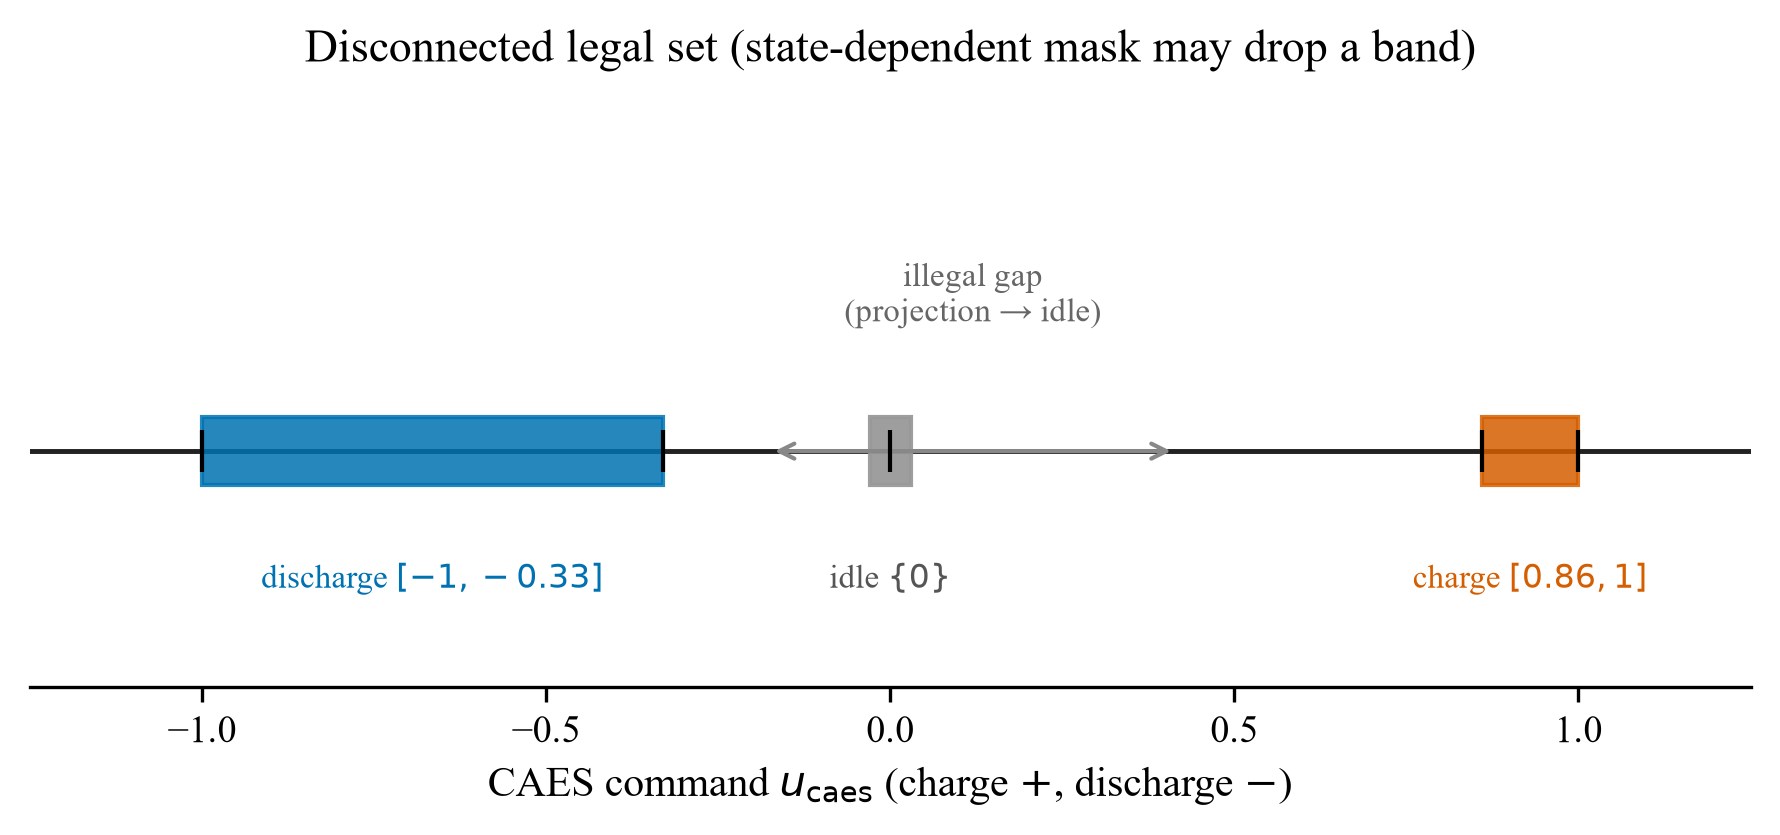
\includegraphics[width=0.88\textwidth]{fig_caes_legal}
\caption{Disconnected legal envelope of the CAES electric command $u_{\mathrm{caes}}$ (discharge band, idle, charge band) together with mode locks that shrink $\mathcal{K}(s)$ and $\mathcal{M}_k(s)$.}
\label{fig:caes-legal}
\end{figure}

\subsection{Reward function for learning}
\label{sec:reward}

With calibration constant $C_{\mathrm{ref}}\approx1.565\times10^{5}$~CNY (rule-controller $p_{95}$ step cash magnitude),
\begin{equation}
r_t^{\mathrm{econ}} = \frac{\Delta J_t^{\mathrm{gen}}}{C_{\mathrm{ref}}}.
\label{eq:recon}
\end{equation}
Potential-based inventory shaping uses the weighted L1 distance $L_{1,t}$ of (battery, gas, hot, cold) relative to episode start:
\begin{equation}
r_t^{\mathrm{shape}}
= \kappa_t \bigl(L_{1,t-1}-L_{1,t}\bigr)
- \kappa_t^{\mathrm{abs}} L_{1,t},
\label{eq:shape}
\end{equation}
with base $\kappa=5$ and a recovery-window scale-up over the last $H=40$~h. At a completed, failure-free terminal step the Cui-style indicator is
\begin{equation}
r_T^{\mathrm{term}}
=
\begin{cases}
B, & L_1^{\mathrm{e}}\le\varepsilon,\\
0, & \text{otherwise},
\end{cases}
\label{eq:term}
\end{equation}
with $B=15$. Missing~\eqref{eq:soc} costs the bonus only; it does not apply a proportional fail penalty, does not rewrite actions and does not invalidate the week. The extrinsic reward is the sum of the three terms
\begin{equation}
r_t^{\mathrm{ext}}
= r_t^{\mathrm{econ}}+r_t^{\mathrm{shape}}+r_t^{\mathrm{term}}.
\label{eq:rext}
\end{equation}
Classical programmes must convexify~\eqref{eq:caes-legal} and the CAES thermo-mechanical coupling; FS-HSAC (Section~\ref{sec:method}) optimises~\eqref{eq:J} by closed-loop interaction with the plant twin under support~\eqref{eq:support}.

% =====================================================================
\section{Solution methodology}
\label{sec:method}
% =====================================================================

The solver is a same-timescale \emph{feasible-support} hybrid soft actor--critic~\cite{haarnoja2018sac}: one plant reward, one state-dependent support, one adopted GiveSafe screen. Mode and magnitude are decided jointly at every one-hour step; with only three CAES modes the soft value can be enumerated exactly. The research question is therefore the current hybrid support $\mathcal{A}(s)$, not a slow inventory sub-goal layer. FS-HSAC is already a two-headed hybrid policy (discrete mode head plus continuous magnitude heads), but it is \emph{not} a multi-timescale hierarchical RL controller in which a high level commits every $c$ hours. When independent slow inventory targets, start-up costs or long-duration options dominate, hierarchical or option methods remain reasonable alternatives; we do not claim that FS-HSAC is universally preferable to them. Figure~\ref{fig:algorithm} summarises the loop; Figure~\ref{fig:action-rep} contrasts projection, fixed-band hybrid decoding and support-consistent decoding.

\begin{figure}[!htbp]
\centering
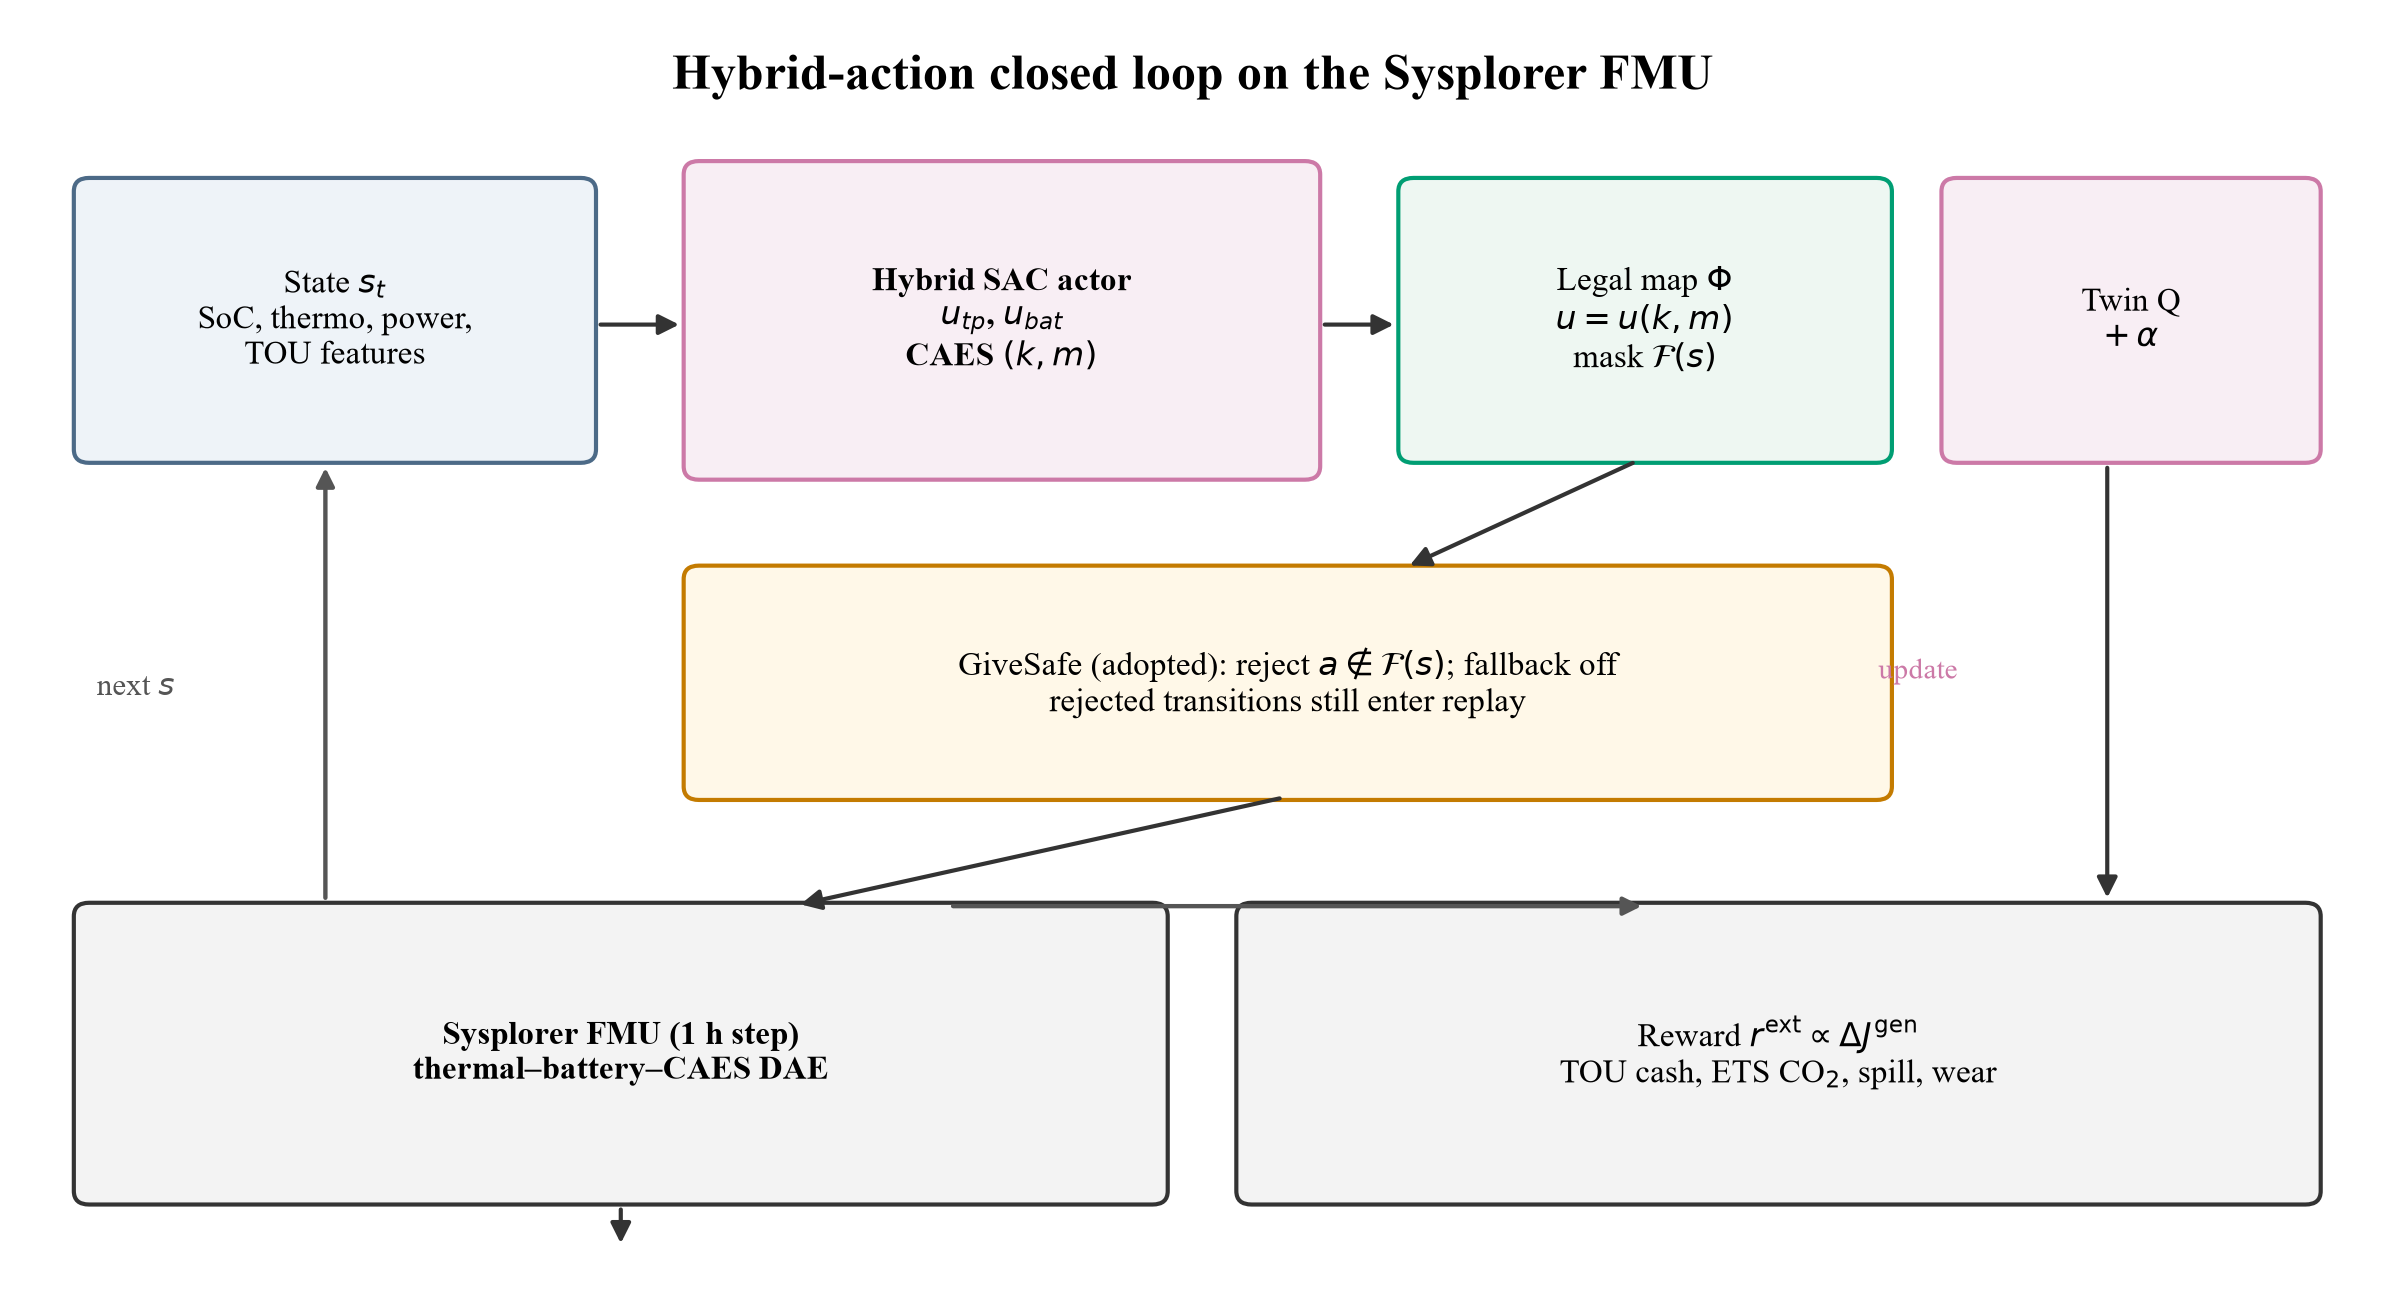
\includegraphics[width=\textwidth]{fig_algorithm}
\caption{FS-HSAC closed loop. The actor issues thermal load rate, battery power and CAES $(\mathrm{mode},\mathrm{magnitude})$ on $\mathcal{A}(s)$ at the same hourly timescale; GiveSafe accepts or rejects before the Sysplorer FMU advances one hour; accepted steps enter the Bellman replay $\mathcal{D}_{\mathrm{B}}$, while rejections train only the residual classifier $C_{\psi}$.}
\label{fig:algorithm}
\end{figure}

\begin{figure}[!htbp]
\centering
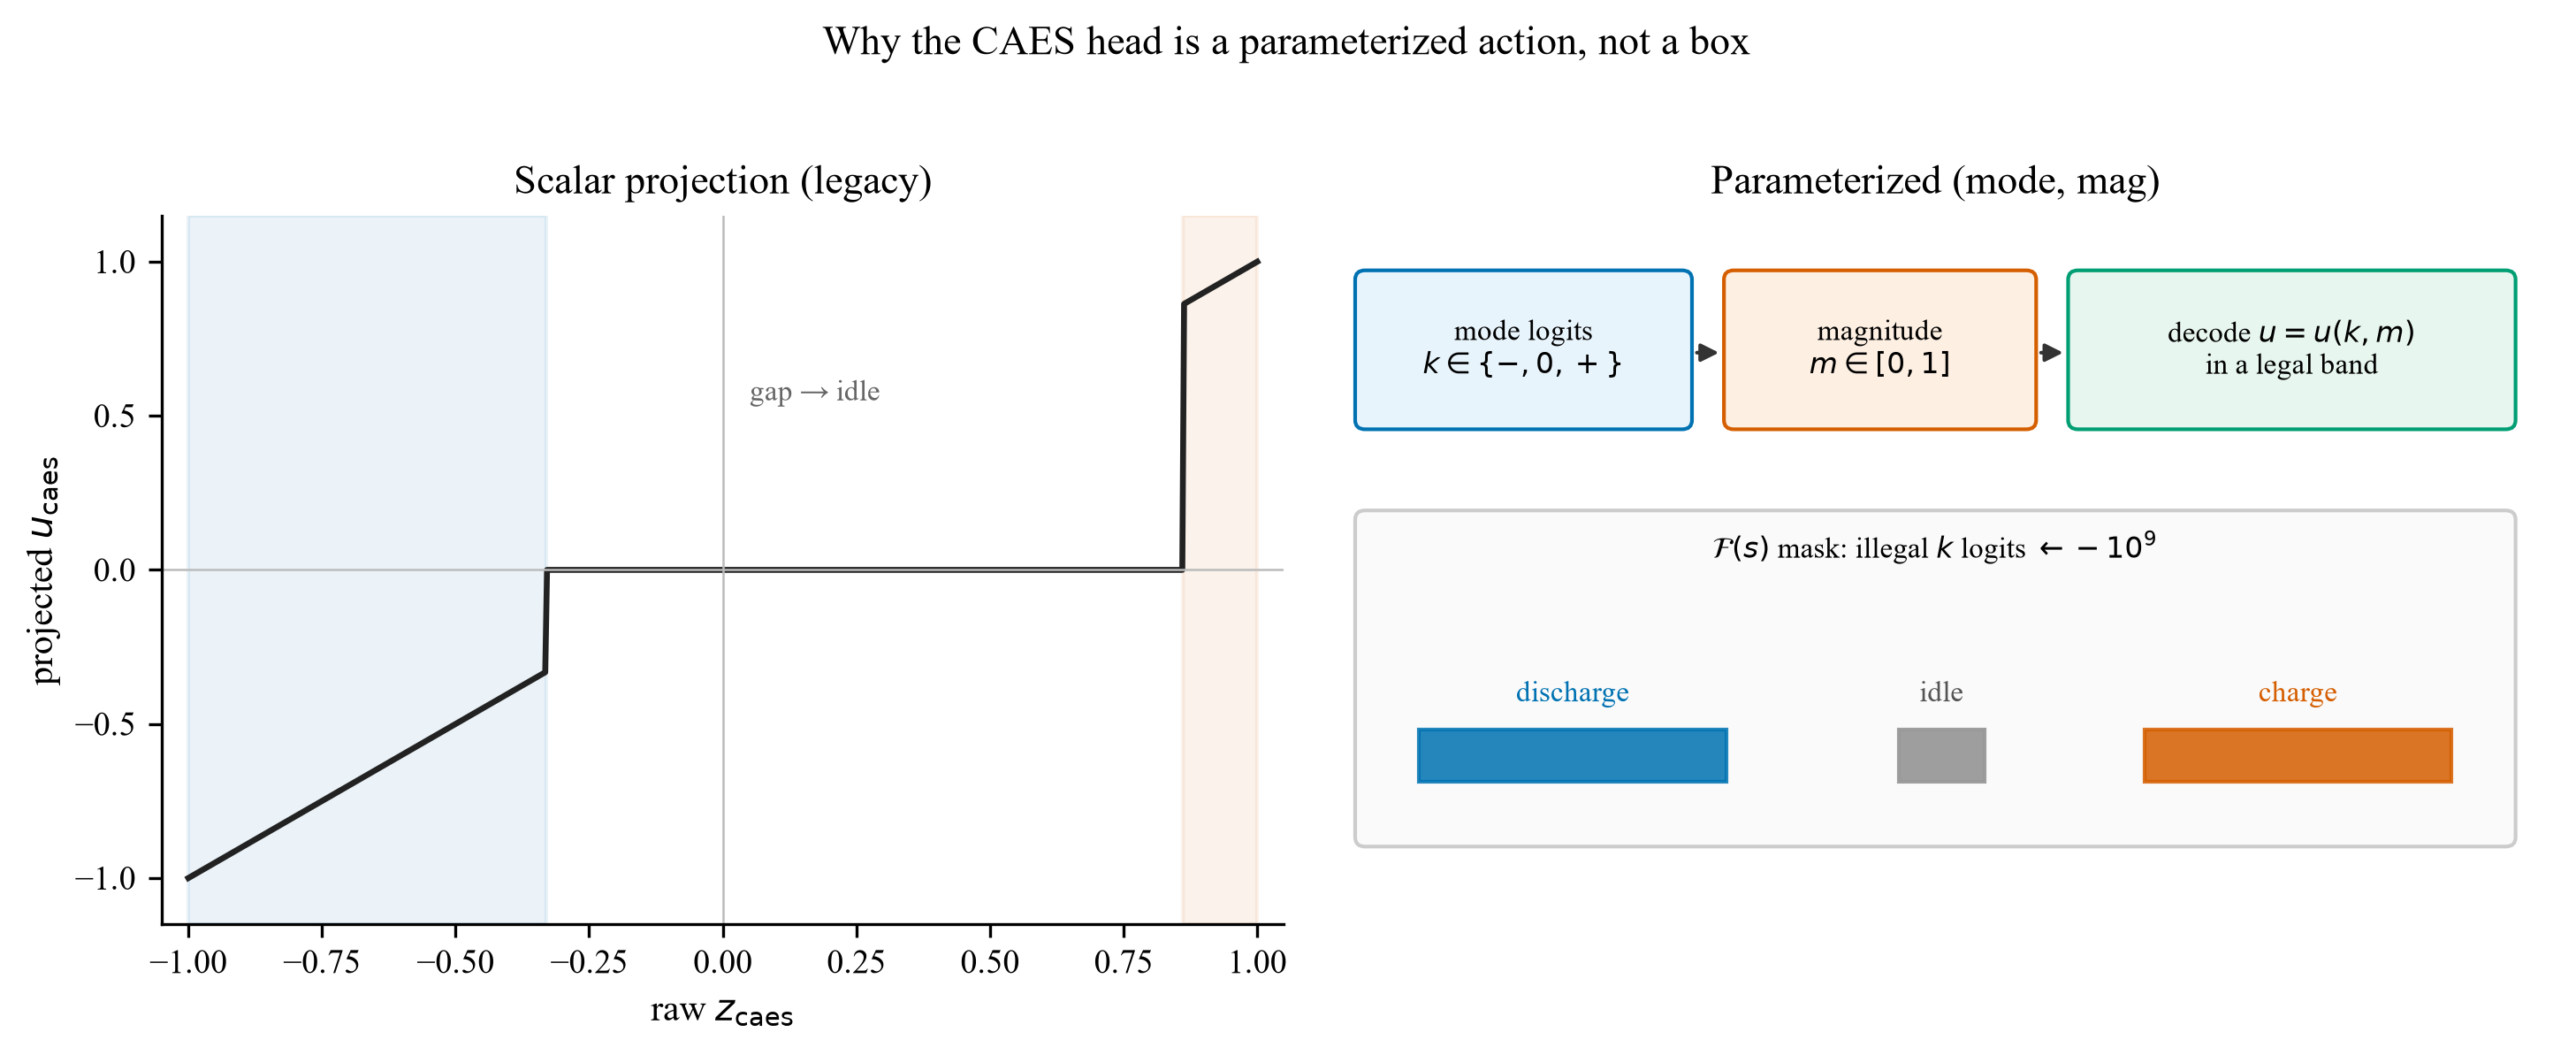
\includegraphics[width=0.95\textwidth]{fig_action_rep}
\caption{Action representation. Left: continuous projection onto~\eqref{eq:caes-legal} can mute charge/discharge into idle. Centre: fixed-band hybrid decoding places magnitude on the static device envelope and clamps after sampling. Right: FS-HSAC maps magnitude through the current interval $\mathcal{M}_k(s)$ with a Jacobian-corrected density.}
\label{fig:action-rep}
\end{figure}
\FloatBarrier

\subsection{Feasible-support hybrid actor}
\label{sec:hybrid-sac}

The hybrid policy factorises as
\begin{equation}
\pi_{\theta}(a^{\mathrm{hyb}}\mid s)
=
\pi_d(k\mid s,\mathcal{K}(s))\,
\pi_c\bigl(u_{\mathrm{tp}},u_{\mathrm{bat}},\mu\mid s,k,\mathcal{M}_k(s)\bigr).
\label{eq:pi-factor}
\end{equation}
Thermal and battery heads use state-dependent Gaussian latents mapped by a sigmoid onto $\mathcal{A}_{\mathrm{tp}}(s)$ and $\mathcal{A}_{\mathrm{bat}}(s)$. The CAES head emits three mode logits $\ell_t\in\mathbb{R}^{3}$ and \emph{separate} discharge/charge magnitude heads. With mask $M(s)$,
\begin{equation}
\tilde\ell_t
=
\ell_t + \log\bigl(M(s)+\varepsilon\bigr)
\quad\text{(illegal modes set to $-\infty$)},
\label{eq:mask}
\end{equation}
yielding a categorical $\pi_d$. For active charge/discharge modes, a Gaussian latent is mapped by sigmoid then affine transform into $\mathcal{M}_k(s)$; the log-density adds both sigmoid and interval Jacobians. Idle contributes no continuous magnitude entropy. Soft actor and critic objectives \emph{enumerate} the three modes exactly (no Gumbel soft-value approximation),
\begin{equation}
\begin{aligned}
J(\theta)
=
\mathbb{E}_{s}\Biggl[
\sum_{k\in\mathcal{K}(s)}\pi_d(k\mid s)\,
\mathbb{E}_{\mu}\Bigl[
Q_{\psi}(s,k,\mu)
-
\alpha_c\log\pi_c(\cdot\mid s,k)
\Bigr]
-
\alpha_d\log\pi_d(k\mid s)
\Biggr],
\end{aligned}
\label{eq:sac-j}
\end{equation}
with dual temperatures $\alpha_d,\alpha_c$ targeting discrete entropy $-\log|\mathcal{K}(s)|$ and continuous entropy scaled by the number of active continuous channels. Twin critics $Q_{\psi_1},Q_{\psi_2}$ take the hybrid argument $(s,u_{\mathrm{tp}},u_{\mathrm{bat}},\mathrm{onehot}(k),\mu)$ rather than a collapsed scalar $u_{\mathrm{caes}}$.

\subsection{Split replay and residual feasibility}
\label{sec:givesafe}

Before every FMU step the controller attempts up to $N_{\mathrm{try}}=64$ samples from $\pi_{\theta}$. A candidate is accepted only if it lies in $\mathcal{F}(s)$. Accepted physical transitions $(s,a,r^{\mathrm{ext}},s')$ enter the Bellman buffer $\mathcal{D}_{\mathrm{B}}$. Rejected proposals never advance the twin and are written only to a feasibility buffer $\mathcal{D}_{\mathrm{F}}$ that trains a residual classifier
\begin{equation}
C_{\psi}(s,a)=\sigma\bigl(f_{\psi}(s,u_{\mathrm{tp}},u_{\mathrm{bat}},\mathrm{onehot}(k),\mu)\bigr)
\approx
\mathbb{P}(\mathrm{accept}\mid s,a).
\label{eq:cpsi}
\end{equation}
Analytic constraints already encoded in $\mathcal{A}(s)$ are not re-learned; $C_{\psi}$ targets residual twin failures. The actor may include a risk penalty $\beta[-\log C_{\psi}(s,a)]$ once unsafe labels exist. With fallback \emph{off}, exhaustion raises \texttt{NoSafeActionFoundError} and the episode is recorded as \texttt{eval\_failed}. GiveSafe follows prior safe-interaction practice~\cite{garcia2015safe,sun2024constrained}; we do not claim a new shield.

\subsection{Ablations and classical baselines}
\label{sec:ablation}

Three learning controls isolate the support design. (i)~\textbf{Projected continuous SAC/TD3:} a single CAES latent $z$ is mapped by
\begin{equation}
u_{\mathrm{caes}}
=
\Pi_{\mathrm{bands}}\bigl(\tanh(z)\bigr),
\label{eq:project}
\end{equation}
where $\Pi_{\mathrm{bands}}$ clamps into the nearest charge/discharge band or to idle~$0$ when $\tanh(z)$ falls in the open gap. (ii)~\textbf{Fixed-band hybrid SAC:} mode masking as in~\eqref{eq:mask} but magnitude decoded onto the static device envelope~\eqref{eq:caes-legal}, with clamp only at evaluation; rejections may be mixed into a single replay (ablation stack). (iii)~\textbf{FS-HSAC-support:} FS-HSAC without the $C_{\psi}$ actor penalty. Classical baselines are six-parameter peak--valley PSO (open-loop week search on the FMU), rolling linprog on an eight-hour linear surrogate, and a rolling MILP with energy linearisation whose modelling omissions are stated in the case-study setup.

\begin{algorithm}[!htbp]
\caption{FS-HSAC with dynamic support, split replay and GiveSafe}
\label{alg:hsac}
\begin{algorithmic}[1]
\Require Actor $\pi_{\theta}$, twin critics, buffers $\mathcal{D}_{\mathrm{B}},\mathcal{D}_{\mathrm{F}}$, classifier $C_{\psi}$, GiveSafe with fallback off
\For{episode $=1,2,\ldots,E_{\max}$}
  \State Reset plant twin on a training-week start; $s\leftarrow s_0$
  \For{$t=0$ to $T-1$}
    \State Build $\mathcal{K}(s),\mathcal{M}_k(s)$; sample $a^{\mathrm{hyb}}\sim\pi_{\theta}(\cdot\mid s)$; decode via~\eqref{eq:decode}
    \State $a^{\star}\leftarrow$ GiveSafe($s,a$; up to $N_{\mathrm{try}}$ resamples)
    \If{no legal $a^{\star}$}
      \State store rejection in $\mathcal{D}_{\mathrm{F}}$; update $C_{\psi}$; \textbf{break} (eval: \texttt{eval\_failed})
    \EndIf
    \State Step FMU with $a^{\star}$; observe $s'$, $r^{\mathrm{ext}}$; store in $\mathcal{D}_{\mathrm{B}}$
    \State Update critics / actor by soft Bellman and~\eqref{eq:sac-j}; adjust $\alpha_d,\alpha_c$; optional $-\log C_{\psi}$ penalty
    \State $s\leftarrow s'$
  \EndFor
\EndFor
\Ensure Learned feasible-support policy $\pi_{\theta}$
\end{algorithmic}
\end{algorithm}

\begin{table}[!htbp]
\centering
\caption{Main FS-HSAC hyperparameters (fair stack).}
\label{tab:hyper}
\scriptsize
\begin{tabular}{@{}llll@{}}
\toprule
Symbol / name & Value & Symbol / name & Value \\
\midrule
$\gamma$ & 0.99 & target $\tau$ & $5\times10^{-3}$ \\
actor / critic lr & $3\times10^{-4}$ & batch size & 256 \\
Bellman / feas.\ buffers & $1\times10^{6}$ each & GiveSafe tries & 64 \\
$\alpha_d,\alpha_c$ & automatic & target $H_c$ & $-3$ (active cont.) \\
feasibility $\beta$ & $0.1$ (when enabled) & algorithm tag & \texttt{fs\_hsac\_v2} \\
$C_{\mathrm{ref}}$ & $1.565\times10^{5}$ CNY & soft-bonus $\varepsilon$ & 0.06 \\
terminal $B$ / fail pen. & 15 / 0 & episode length $T$ & 168 h \\
reported seed & $0$ & training episodes $E_{\max}$ & $5\times10^{3}$ \\
observation dim & 166 & hybrid act.\ $(u_{\mathrm{tp}},u_{\mathrm{bat}},k,\mu)$ & --- \\
\bottomrule
\end{tabular}
\end{table}
\FloatBarrier

% =====================================================================
\section{Case study setup}
\label{sec:setup}
% =====================================================================

The numerical study is a fair \emph{weekly} protocol on the same Sysplorer FMU, TOU table and resource files. Each episode lasts \(T=168\)~h. The 8760~h calendar only supplies rotating week-start times; energy inventories are re-initialised at each reset. Continuous-year carry is an appendix protocol only and is \emph{not} used to claim annual RL superiority. Three seasons follow common hierarchical multi-energy windowing~\cite{cui2025ghtd3}: winter trains on weeks \(0\)--\(4\) and evaluates week~\(5\); transition trains on weeks \(13\)--\(17\) and evaluates week~\(18\); summer trains on weeks \(26\)--\(30\) and evaluates week~\(31\). All learning agents use seed~\(0\) and \(E_{\max}=5\times10^{3}\) episodes (\(\approx 8.4\times10^{5}\) valid steps). Hyperparameters are Table~\ref{tab:hyper}.

\paragraph{Methods.}
The mainline is \textbf{FS-HSAC}; ablations are \textbf{projected continuous SAC/TD3}, \textbf{fixed-band hybrid SAC}, and \textbf{FS-HSAC-support} (no $C_{\psi}$ penalty). Classical controls are six-parameter peak--valley \textbf{PSO}, rolling \textbf{linprog}, and rolling \textbf{MILP}. GiveSafe stays on for every learning agent; fallback is \emph{off}. Held-out evaluation uses the same rule for every method. Rows that are still missing after the results gate are left blank and are not filled from older observation-dimension archives.

\paragraph{Metrics.}
Primary ranking uses the full-week comprehensive monetary objective~\eqref{eq:J}: report $J^{\mathrm{gen}}$ and $CC=-J^{\mathrm{gen}}$ only when $\texttt{valid\_steps}=168$. Cost breakdown columns expose cash, carbon, $C^{CUT}$, degradation, CAES startup and soft grid-contract charges (fields in \texttt{train\_result.json}/\texttt{kpi}). Independent physical KPIs are reported in parallel and never replace $CC$ as the economic ranking key:
\begin{itemize}
  \item \emph{Renewable uptake:} curtailment MWh, rate $E^{\mathrm{curt}}/E^{\mathrm{RES,avail}}$, utilisation.
  \item \emph{Flexibility / grid friendliness:} contract excess MWh and violation hours, $|P^{\mathrm{grid}}|_{\max}$, peak--valley and ramp of interchange (1~h resolution; no claim of sub-hourly response).
  \item \emph{Reliability / executability:} unserved MWh, valid steps, FMU failures, GiveSafe rejects, terminal inventory diagnostics.
  \item \emph{Online compute:} mean/p95/max decision time; for rolling MILP/linprog also timeout and fail counts.
\end{itemize}
Hours survived and \texttt{eval\_failed} remain a separate executability table (Table~\ref{tab:run}); truncated sums are never compared with full weeks. Battery/gas SoC trajectories are qualitative; the week-end indicator~\eqref{eq:term} is a soft bonus, not a ranking KPI. Declaration rule: lowest $CC$ is ``economically best''; better curtailment or fewer contract excesses is stated only on that axis; ``overall better'' is reserved for weak Pareto dominance on $CC$, curtailment and reliability together.

% =====================================================================
\section{Simulation results}
\label{sec:results}
% =====================================================================

\subsection{Executability under the hard filter}

\emph{Provisional note.} Tables in this section still quote the pre--FS-HSAC \texttt{seasonal\_v1} seed-$0$ archive (projected TD3 / fixed-band hybrid SAC / PSO / linprog). They will be replaced by FS-HSAC rows once \texttt{docs/fs\_hsac\_results\_gate.md} passes; blank FS-HSAC cells are intentional.

Table~\ref{tab:run} reports executability under GiveSafe with fallback off. Projected continuous TD3 aborts at 13/5/76~h across winter/transition/summer. The archived fixed-band hybrid SAC records \texttt{eval\_failed} on winter and transition held-out weeks; summer is missing. PSO finishes winter (168~h) but truncates transition (143~h) and summer (117~h). Rolling linprog finishes all three seasons on the FMU first-step execution protocol. These facts are executability, not cash.

\begin{table}[!htbp]
\centering
\caption{Executability on the held-out week (seed~$0$, \texttt{seasonal\_v1}, GiveSafe fallback off). Hours are valid FMU steps. FS-HSAC rows are reserved for the post-gate archive; ``hybrid SAC'' below denotes the fixed-band ablation.}
\label{tab:run}
\scriptsize
\begin{tabular}{lllr}
\toprule
Season & Method & Status & Hours \\
\midrule
Winter & hybrid SAC & eval\_failed & --- \\
Winter & proj.\ TD3 & completed & 13 \\
Winter & PSO & completed & 168 \\
Winter & linprog & completed & 168 \\
Transition & hybrid SAC & eval\_failed & --- \\
Transition & proj.\ TD3 & completed & 5 \\
Transition & PSO & completed & 143 \\
Transition & linprog & completed & 168 \\
Summer & hybrid SAC & missing & --- \\
Summer & proj.\ TD3 & completed & 76 \\
Summer & PSO & completed & 117 \\
Summer & linprog & completed & 168 \\
\bottomrule
\end{tabular}\\[2pt]
{\footnotesize SAC \texttt{eval\_failed}: \texttt{NoSafeActionFoundError} after 64 GiveSafe attempts. Hours $<168$: env terminated on forbidden/invalid command.}
\end{table}
\FloatBarrier

\subsection{Same-horizon economics}

\(R\) and \(J^{\mathrm{gen}}\) accumulate by the hour. Ranking a truncated sum against a 168~h sum would treat survival time as cash. Table~\ref{tab:econ} therefore keeps only \(\texttt{valid\_steps}=168\) and ranks by comprehensive cost $CC=-J^{\mathrm{gen}}$ (equivalently $J^{\mathrm{gen}}$). On the present pre-gate archive the closed-loop learning methods do not yet contribute a full-week FS-HSAC cell; fixed-band hybrid SAC likewise has no full-week cell. Winter economics are therefore PSO versus linprog (both 168~h): PSO \(R=102.7\), \(J^{\mathrm{gen}}=14.36\times10^{6}$~CNY versus linprog \(R=60.0\), \(J^{\mathrm{gen}}=10.19\times10^{6}$~CNY. Transition and summer economic columns contain linprog only among completed main-matrix methods. Incomplete DRL/PSO weeks do not enter Table~\ref{tab:econ}.

\begin{table}[!htbp]
\centering
\caption{Full-week economics (seed~$0$, \texttt{seasonal\_v1}). Only \(\texttt{valid\_steps}=168\). Primary column $J^{\mathrm{gen}}$ ($10^{6}$~CNY) is the comprehensive objective~\eqref{eq:J}; $E^{\mathrm{th}}$ and battery throughput in MWh. Soft week-end inventory bonus is inside $R$, not a separate column.}
\label{tab:econ}
\scriptsize
\begin{tabular}{llrrrr}
\toprule
Season & Method & $R$ & $J^{\mathrm{gen}}$ & $E^{\mathrm{th}}$ & Bat.\ thr. \\
\midrule
Winter & PSO & 102.7 & 14.36 & 14174 & 347 \\
Winter & linprog & 60.0 & 10.19 & 20818 & 5238 \\
Transition & linprog & 13.2 & 2.66 & 21615 & 4288 \\
Summer & linprog & 11.6 & 3.26 & 20745 & 3791 \\
\bottomrule
\end{tabular}
\end{table}
\FloatBarrier

\subsection{Renewable uptake, flexibility and reliability}
\label{sec:kpi-physics}

After the results gate, companion tables report curtailment MWh/rate, contract excess and violation hours, interchange peak--valley/ramp, unserved energy, and decision-time statistics for the same full-week rows as Table~\ref{tab:econ}. These axes do not override $CC$: a method with lower curtailment but higher $CC$ is described as a Pareto trade-off induced by prices and constraints, not as ``smarter'' than a solver. Mechanism ablation (full thermal--BESS--CAES versus lock-CAES under identical forecast and~\eqref{eq:J}) attributes $\Delta CC$, $\Delta E^{\mathrm{curt}}$ and interchange changes to device complementarity rather than to a single synthetic synergy index.

\subsection{Sensitivity and Pareto language}
\label{sec:sensitivity-rules}

Sensitivity axes include carbon price, feasibility-margin scale, CAES capacity, curtailment price $\nu_{\mathrm{curt}}$ and contract price $\nu_{\mathrm{grid}}$ (protocol in the sensitivity notes). If MILP records lower $CC$ but higher curtailment, the text reports the price-driven trade-off and verifies it on the curtailment/contract sweeps; it does not reinterpret that gap as an RL forecast advantage. The main matrix shares perfect forecast across methods.
\subsection{Scheduling traces and surrogate gap}

Closed-loop power-balance plots show only evaluations that completed \(T=168\)~h. Truncated rollouts and SAC \texttt{eval\_failed} stay in Table~\ref{tab:run}. On the present main matrix the full-week electric stackplot available for discussion is rolling linprog (Fig.~\ref{fig:bal-t} shows the transition week). Fig.~\ref{fig:soc-mat} plots battery and CAES gas SoC on full-horizon weeks. Training curves for archived TD3/SAC runs mix exploration noise and rotating weeks; they are not held-out scores (Fig.~\ref{fig:training}).

\begin{figure}[!htbp]
\centering
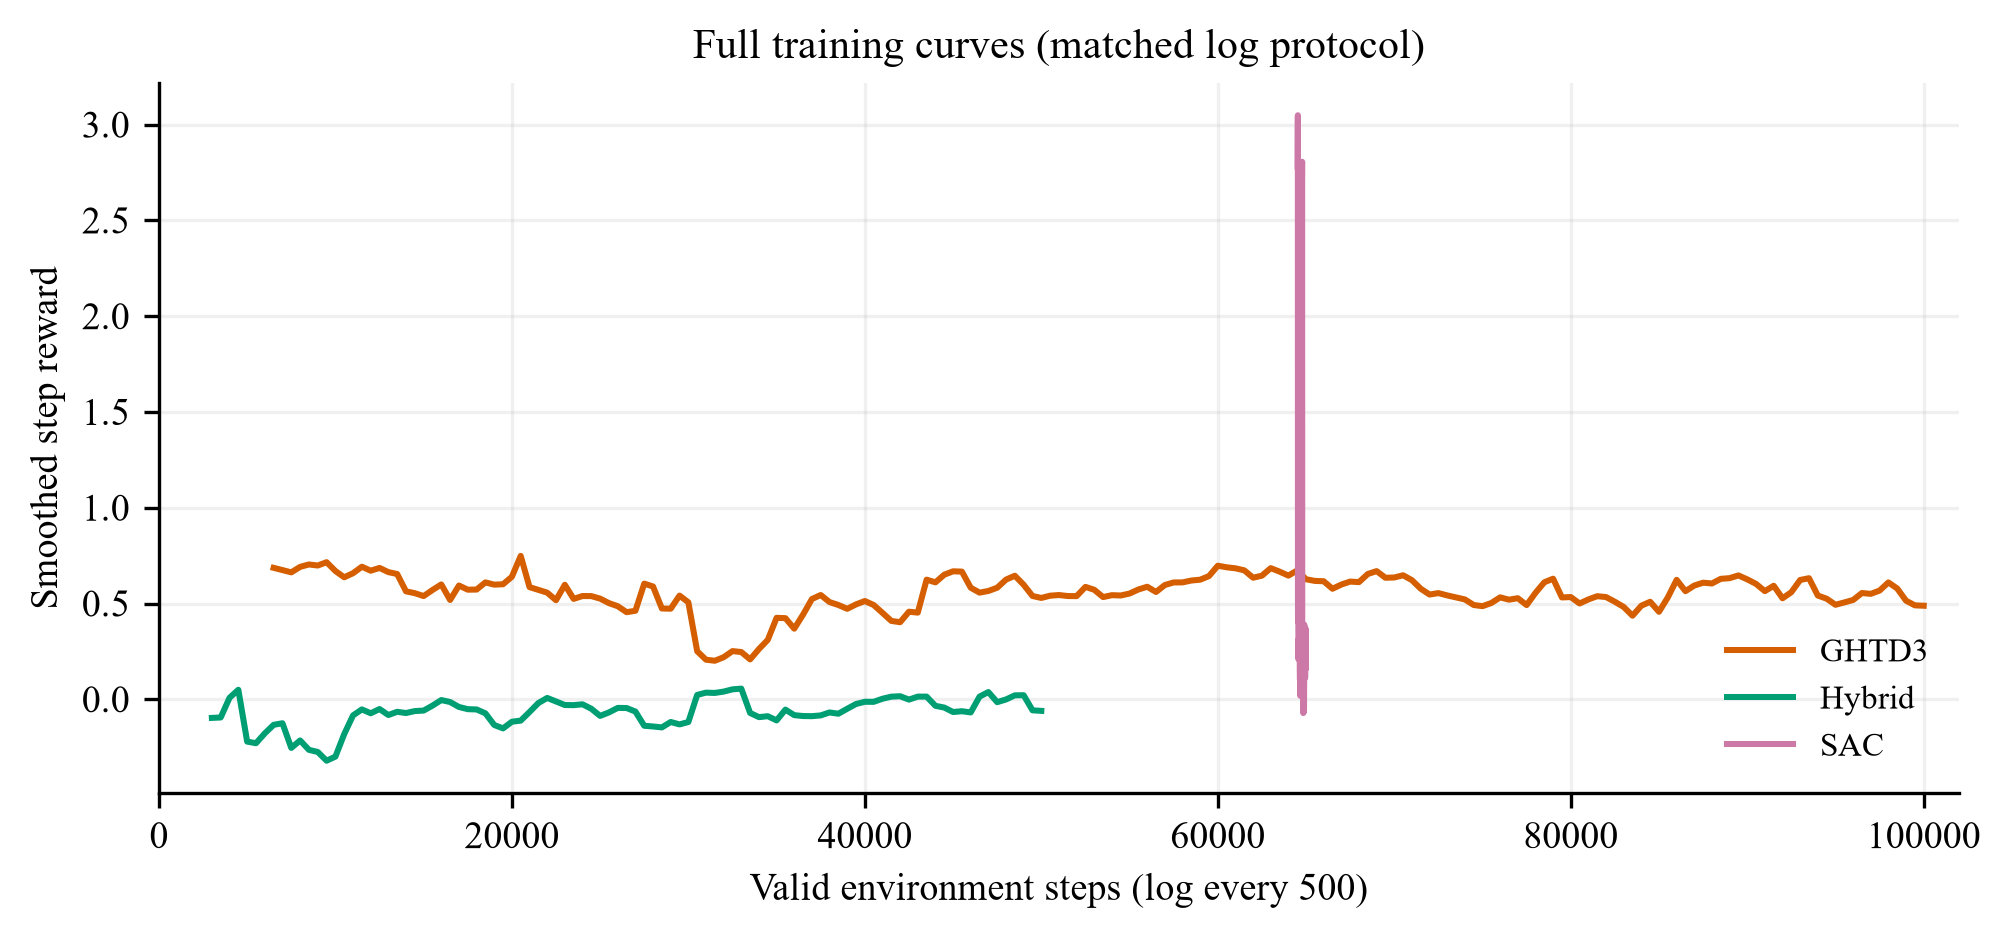
\includegraphics[width=\textwidth]{fig_training}
\caption{Training curves for archived seasonal runs (seed~$0$). Full-week held-out scores are Table~\ref{tab:econ}; hours survived are Table~\ref{tab:run}.}
\label{fig:training}
\end{figure}

\begin{figure}[!htbp]
\centering
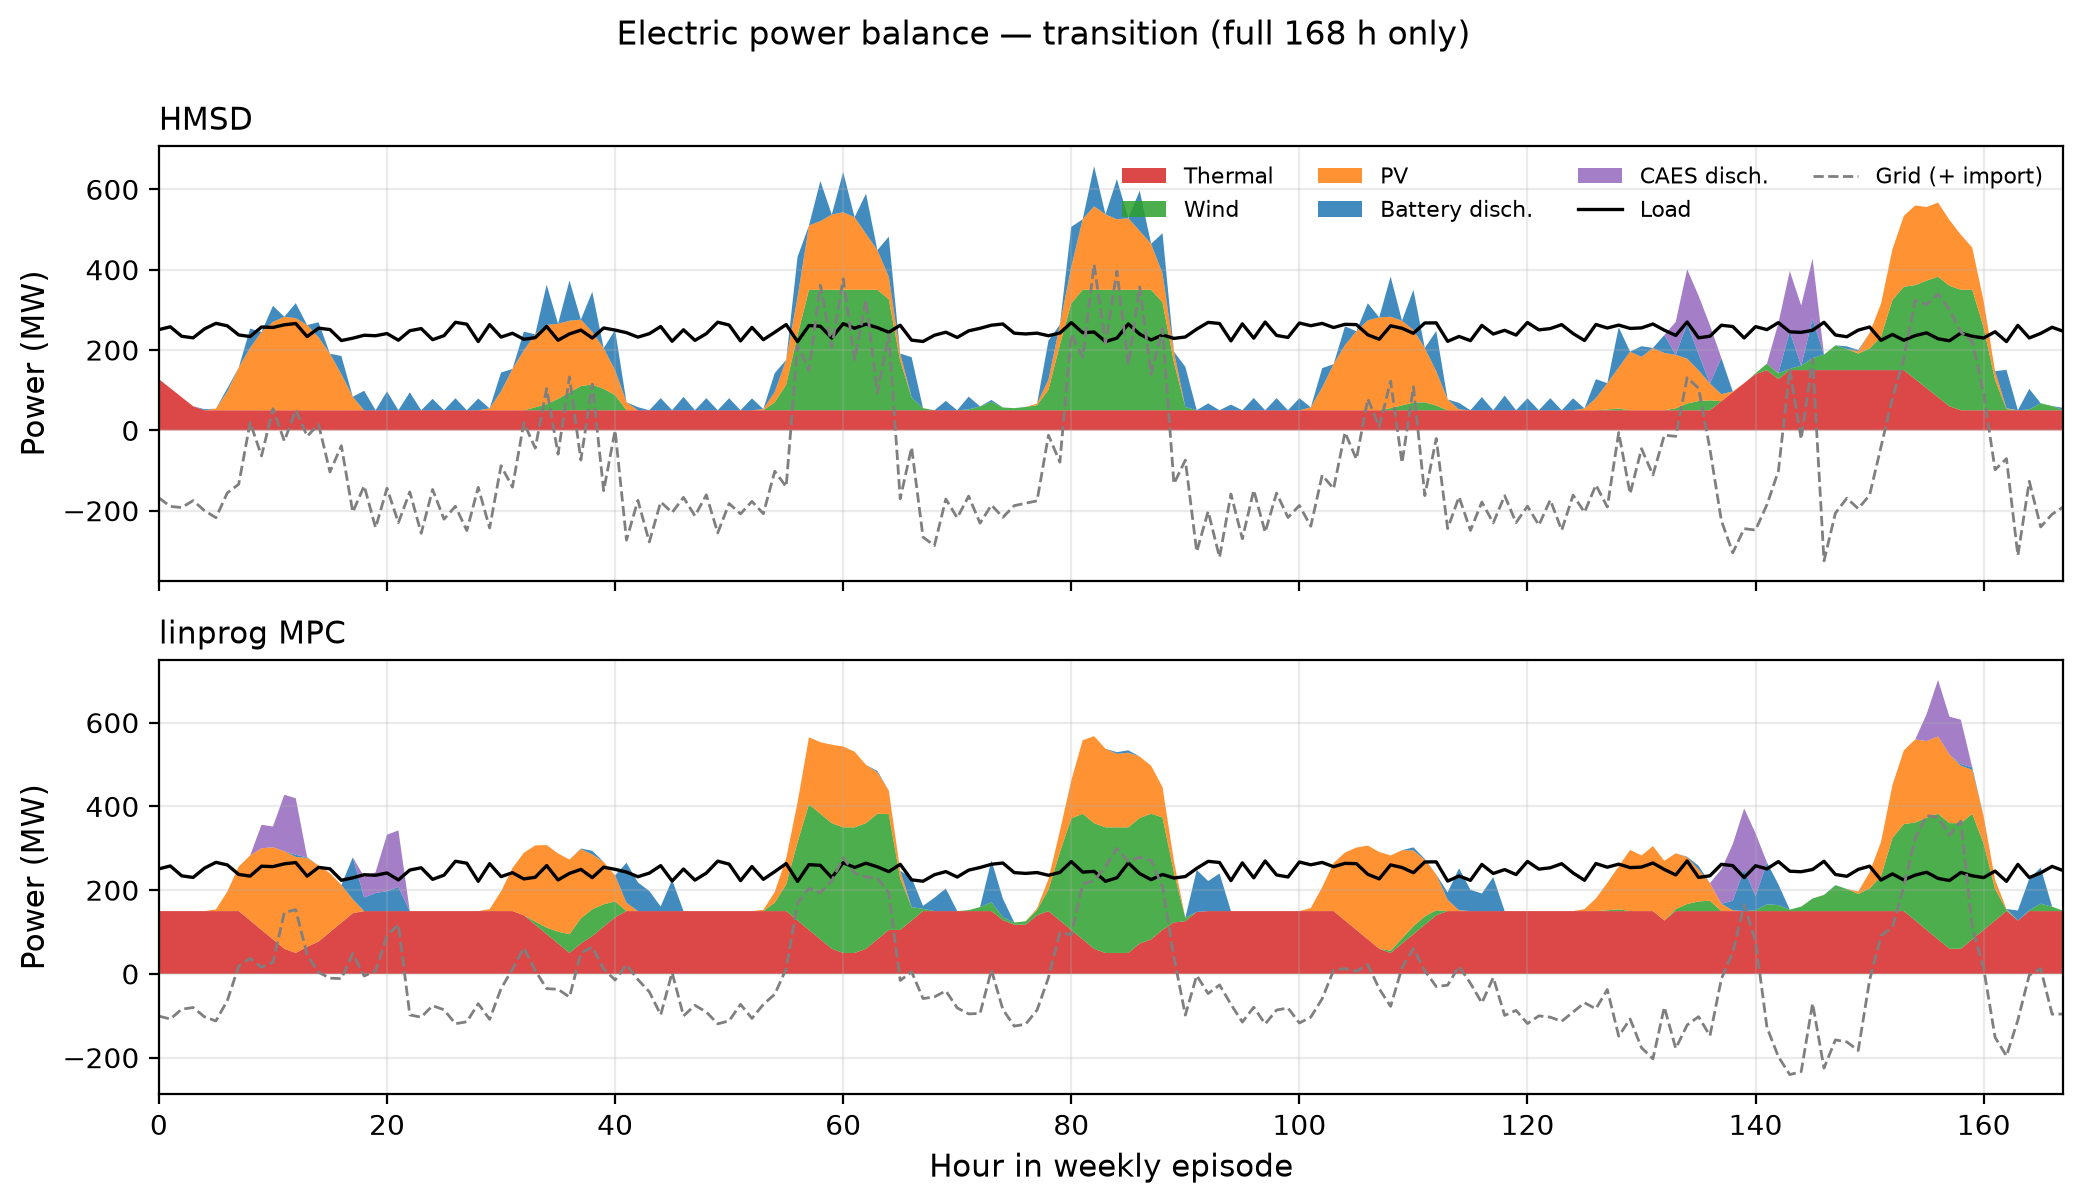
\includegraphics[width=\textwidth]{fig_balance_transition}
\caption{Transition held-out week electric power balance (seed~$0$), full \(168\)~h closed-loop traces for main-matrix linprog.}
\label{fig:bal-t}
\end{figure}

\begin{figure}[!htbp]
\centering
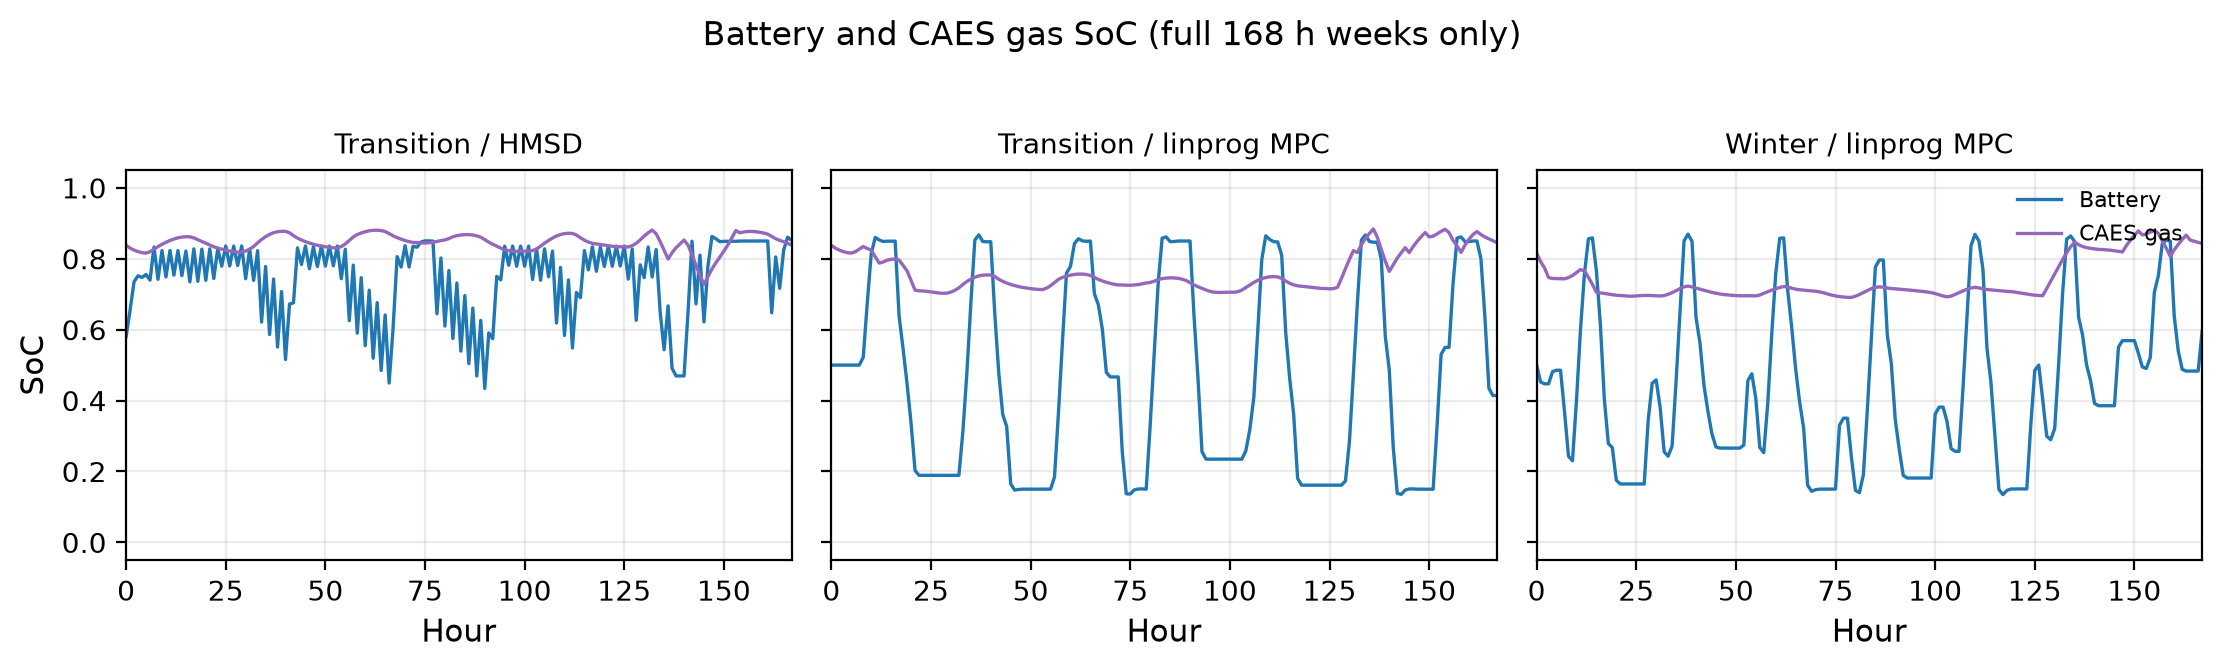
\includegraphics[width=\textwidth]{fig_soc_seasons}
\caption{Battery and CAES gas SoC on full \(168\)~h held-out weeks (seed~$0$); qualitative inventory behaviour, not a ranking KPI.}
\label{fig:soc-mat}
\end{figure}
\FloatBarrier

\begin{table}[!htbp]
\centering
\caption{Same-horizon mechanism split (seed~$0$, \texttt{seasonal\_v1}, \(168\)~h only). \(J^{\mathrm{gen}}\), carbon and cycle wear in $10^{6}$~CNY; thermal / battery in MWh.}
\label{tab:mech}
\scriptsize
\begin{tabular}{llrrrrr}
\toprule
Season & Method & $J^{\mathrm{gen}}$ & Carbon & Wear & $E^{\mathrm{th}}$ & Bat.\ thr. \\
\midrule
Winter & PSO & 14.36 & --- & --- & 14174 & 347 \\
Winter & linprog & 10.19 & 0.088 & 0.001 & 20818 & 5238 \\
Transition & linprog & 2.66 & 0.415 & 0.001 & 21615 & 4288 \\
Summer & linprog & 3.26 & 0.290 & 0.000 & 20745 & 3791 \\
\bottomrule
\end{tabular}
\end{table}
\FloatBarrier

\paragraph{Why PSO and rolling linprog are not FS-HSAC.}
PSO tunes a six-dimensional peak--valley heuristic scored by full FMU weeks with open-loop parameters; linprog rolls an eight-hour linear surrogate. Winter PSO outscores linprog on the same 168~h cell; that contrast is classical search versus convex surrogate, not evidence that FS-HSAC already wins cash. Incomplete weeks are not used to extend claims. The baselines remain diagnostics of the plant object, not global bounds on the FMU.

\subsection{Discussion}
\label{sec:support}

Tables~\ref{tab:econ}--\ref{tab:run} remain a single-seed pre--FS-HSAC snapshot (obs~$=166$). Economics are same-horizon only. Executability is separate: projected TD3 aborts early; fixed-band hybrid SAC has not closed a held-out week on this seed under GiveSafe without fallback. FS-HSAC seasonal numbers are withheld until the results gate. Continuous-year cold-tank viability and intensity carbon books stay in Appendix~\ref{app:annual-carbon}; they do \emph{not} support an ``8760~h safe and best economics'' claim for RL.

Limitations: one seed pending multi-seed FS-HSAC runs; dynamic magnitude intervals mix twin physics with oracle margins; weekly-reset protocol for the main text; $C_{\psi}$ is used as a risk penalty rather than a second hard gate in front of GiveSafe.

% =====================================================================
\section{Conclusion}
\label{sec:conclusion}
% =====================================================================

Weekly thermal--battery--CAES dispatch under TOU prices and a National ETS carbon price is a comprehensive monetary problem whose hybrid actions live on a state-dependent support $\mathcal{A}(s)$. This paper formalises that support---admissible modes $\mathcal{K}(s)$ and mode-conditioned intervals $\mathcal{M}_k(s)$---and proposes FS-HSAC, a same-timescale hybrid policy with exact mode enumeration, dual temperatures, residual feasibility learning and an adopted GiveSafe shield on an FMI-exported Sysplorer twin. On the provisional pre-gate archive, same-horizon winter economics favour PSO over rolling linprog among completed methods; projected continuous TD3 aborts early and fixed-band hybrid SAC can fail to find a legal action without fallback---executability facts, not truncated-sum cash. Full-week FS-HSAC economics will replace the placeholder tables after the shared results gate. The contribution is the plant object, the support formalisation and the FS-HSAC solver---not a claim that FMI itself is novel, that hierarchical RL is inapplicable, or that RL unconditionally dominates MILP.

\section*{Acknowledgments}

Mengxi system-level boundaries and real-time nodal prices used in related cross-domain studies were provided through the AI4E track of the World Scientific Intelligence Competition; numerical weather prediction fields were supplied by TJ Weather. The authors gratefully acknowledge the organisers and data providers.

\section*{Data availability}

Plant model parameters, TOU reconstruction data and evaluation protocols are available from the authors upon reasonable request, subject to competition data-access rules where applicable.

% =====================================================================
\appendix
\section{Continuous-year viability and intensity carbon accounting}
\label{app:annual-carbon}
% =====================================================================

This appendix records implementation protocols that must \emph{not} be read as ``RL is 8760~h safe and economically optimal.''

\paragraph{Disconnected CAES set.}
Figure~\ref{fig:caes-set} recalls a schematic continuous projection onto the charge / idle / discharge bands (the main-text legal set is Fig.~\ref{fig:caes-legal}).

\begin{figure}[!htbp]
\centering
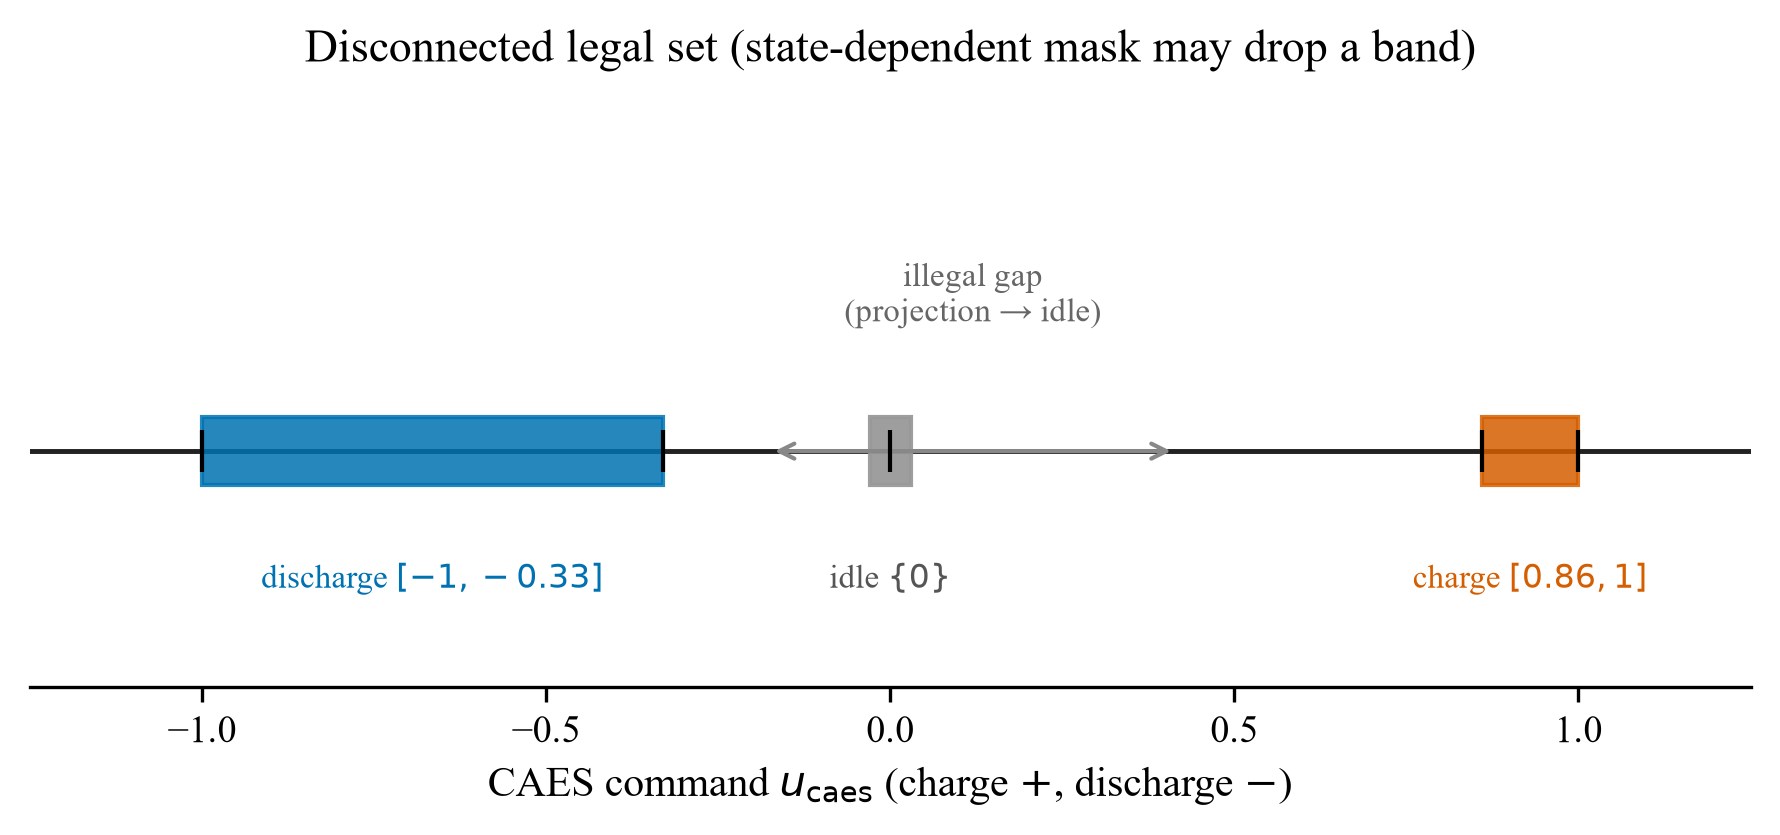
\includegraphics[width=0.88\textwidth]{fig_caes_feasible_set}
\caption{Disconnected legal set of the continuous CAES command and a schematic projection from an illegal raw proposal onto a feasible band (ablation view).}
\label{fig:caes-set}
\end{figure}

\paragraph{Cold-tank transition guard.}
A sign error in the cold-tank mass balance of the one-step feasibility oracle caused continuous annual rollouts to assert-fail near $1276$~h for learning agents. After flipping the cold-tank guard and re-fitting transition coefficients, a rule / B0-style policy can complete $8760$~h (Fig.~\ref{fig:cold}). That fact is a twin-viability check; it is not evidence that hybrid SAC or projected TD3 already delivers annual closed-loop optimality.

\begin{figure}[!htbp]
\centering
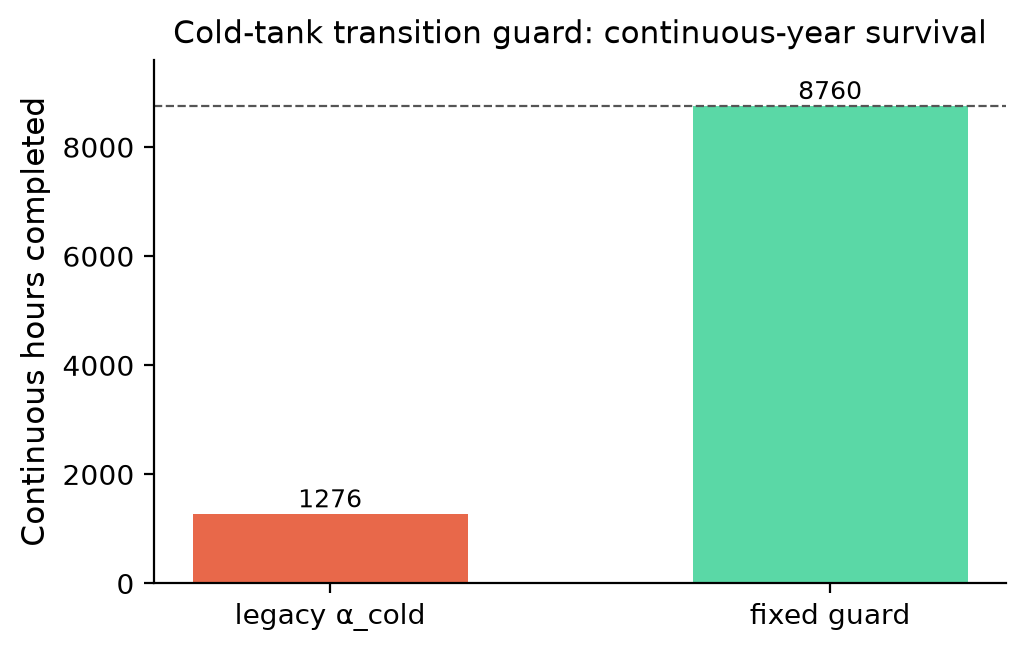
\includegraphics[width=0.72\textwidth]{fig_cold_tank_guard}
\caption{Continuous-year survival before and after correcting the cold-tank transition guard.}
\label{fig:cold}
\end{figure}

\begin{figure}[!htbp]
\centering
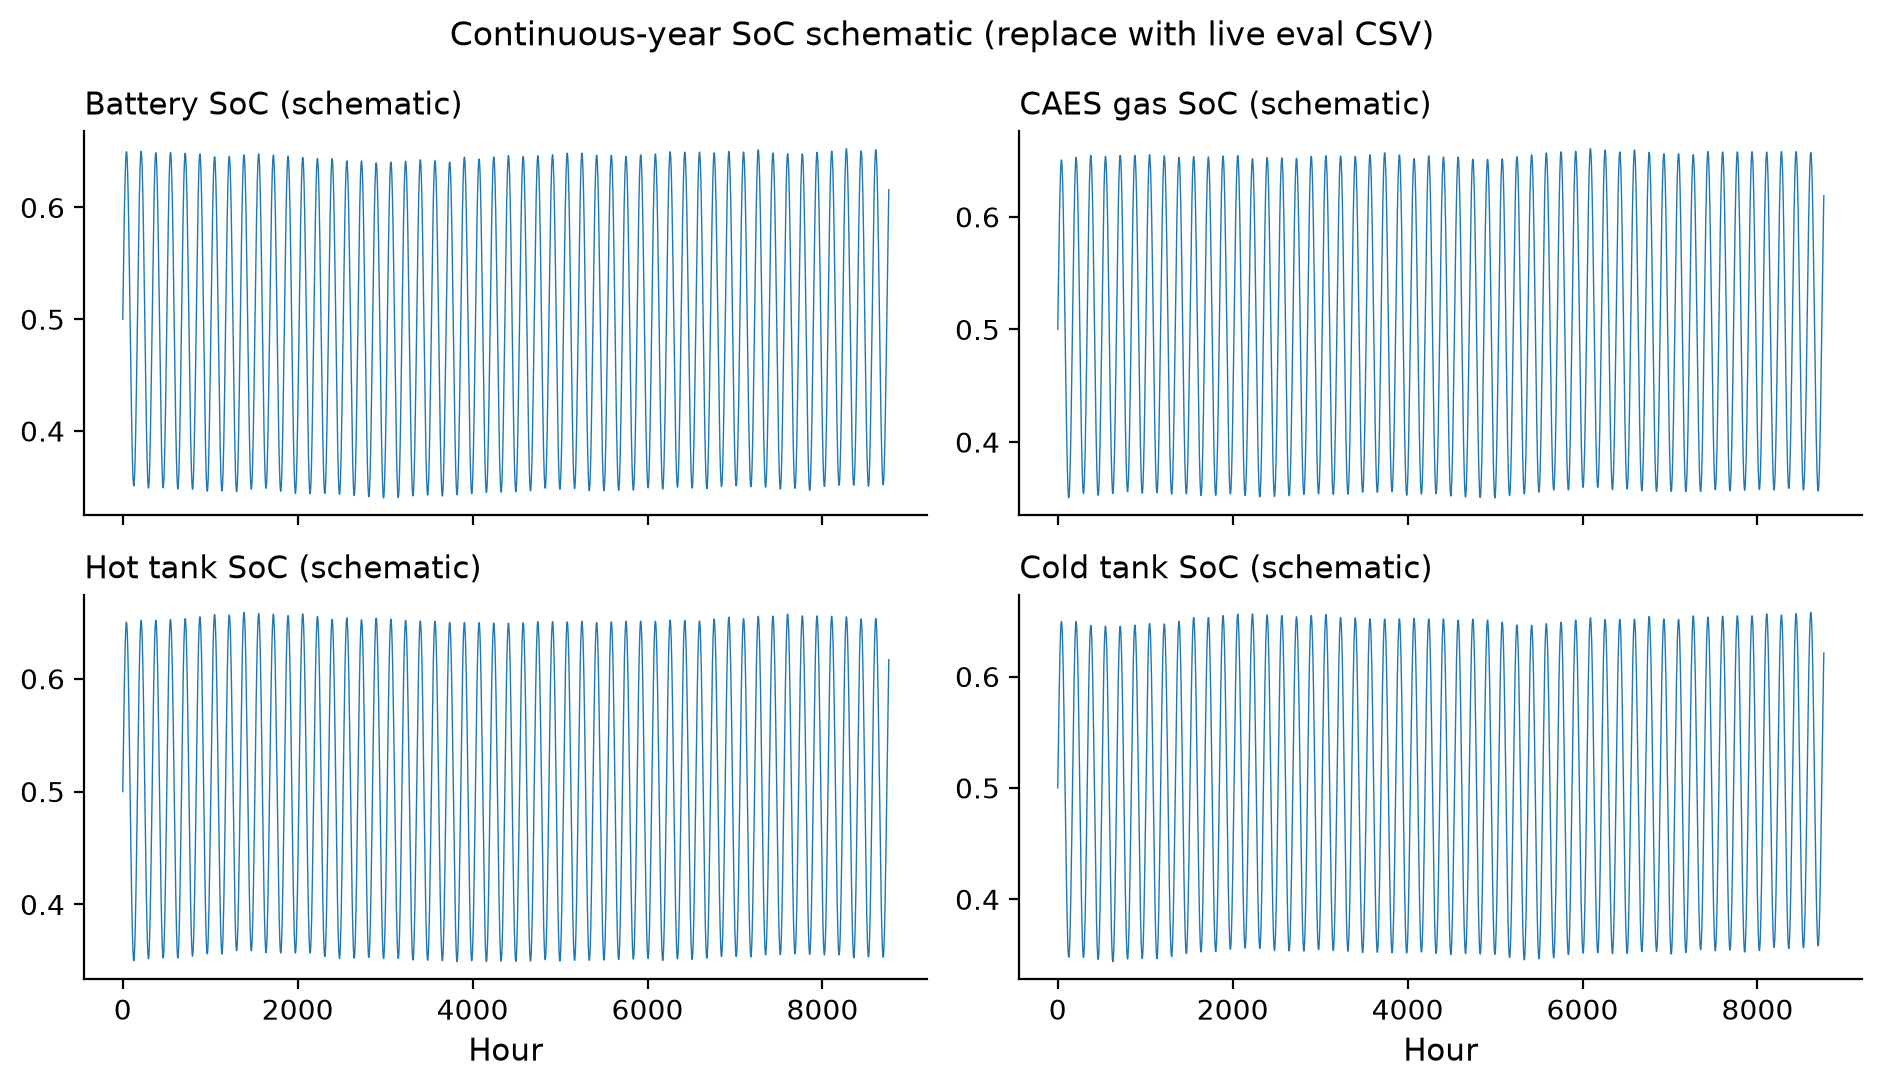
\includegraphics[width=\textwidth]{fig_continuous_year_soc}
\caption{Illustrative continuous-year SoC trajectories (battery, gas, hot and cold tanks). Live evaluation CSVs replace the schematic when continuous annual evals are archived under \texttt{runs/}.}
\label{fig:cont-soc}
\end{figure}

\begin{figure}[!htbp]
\centering
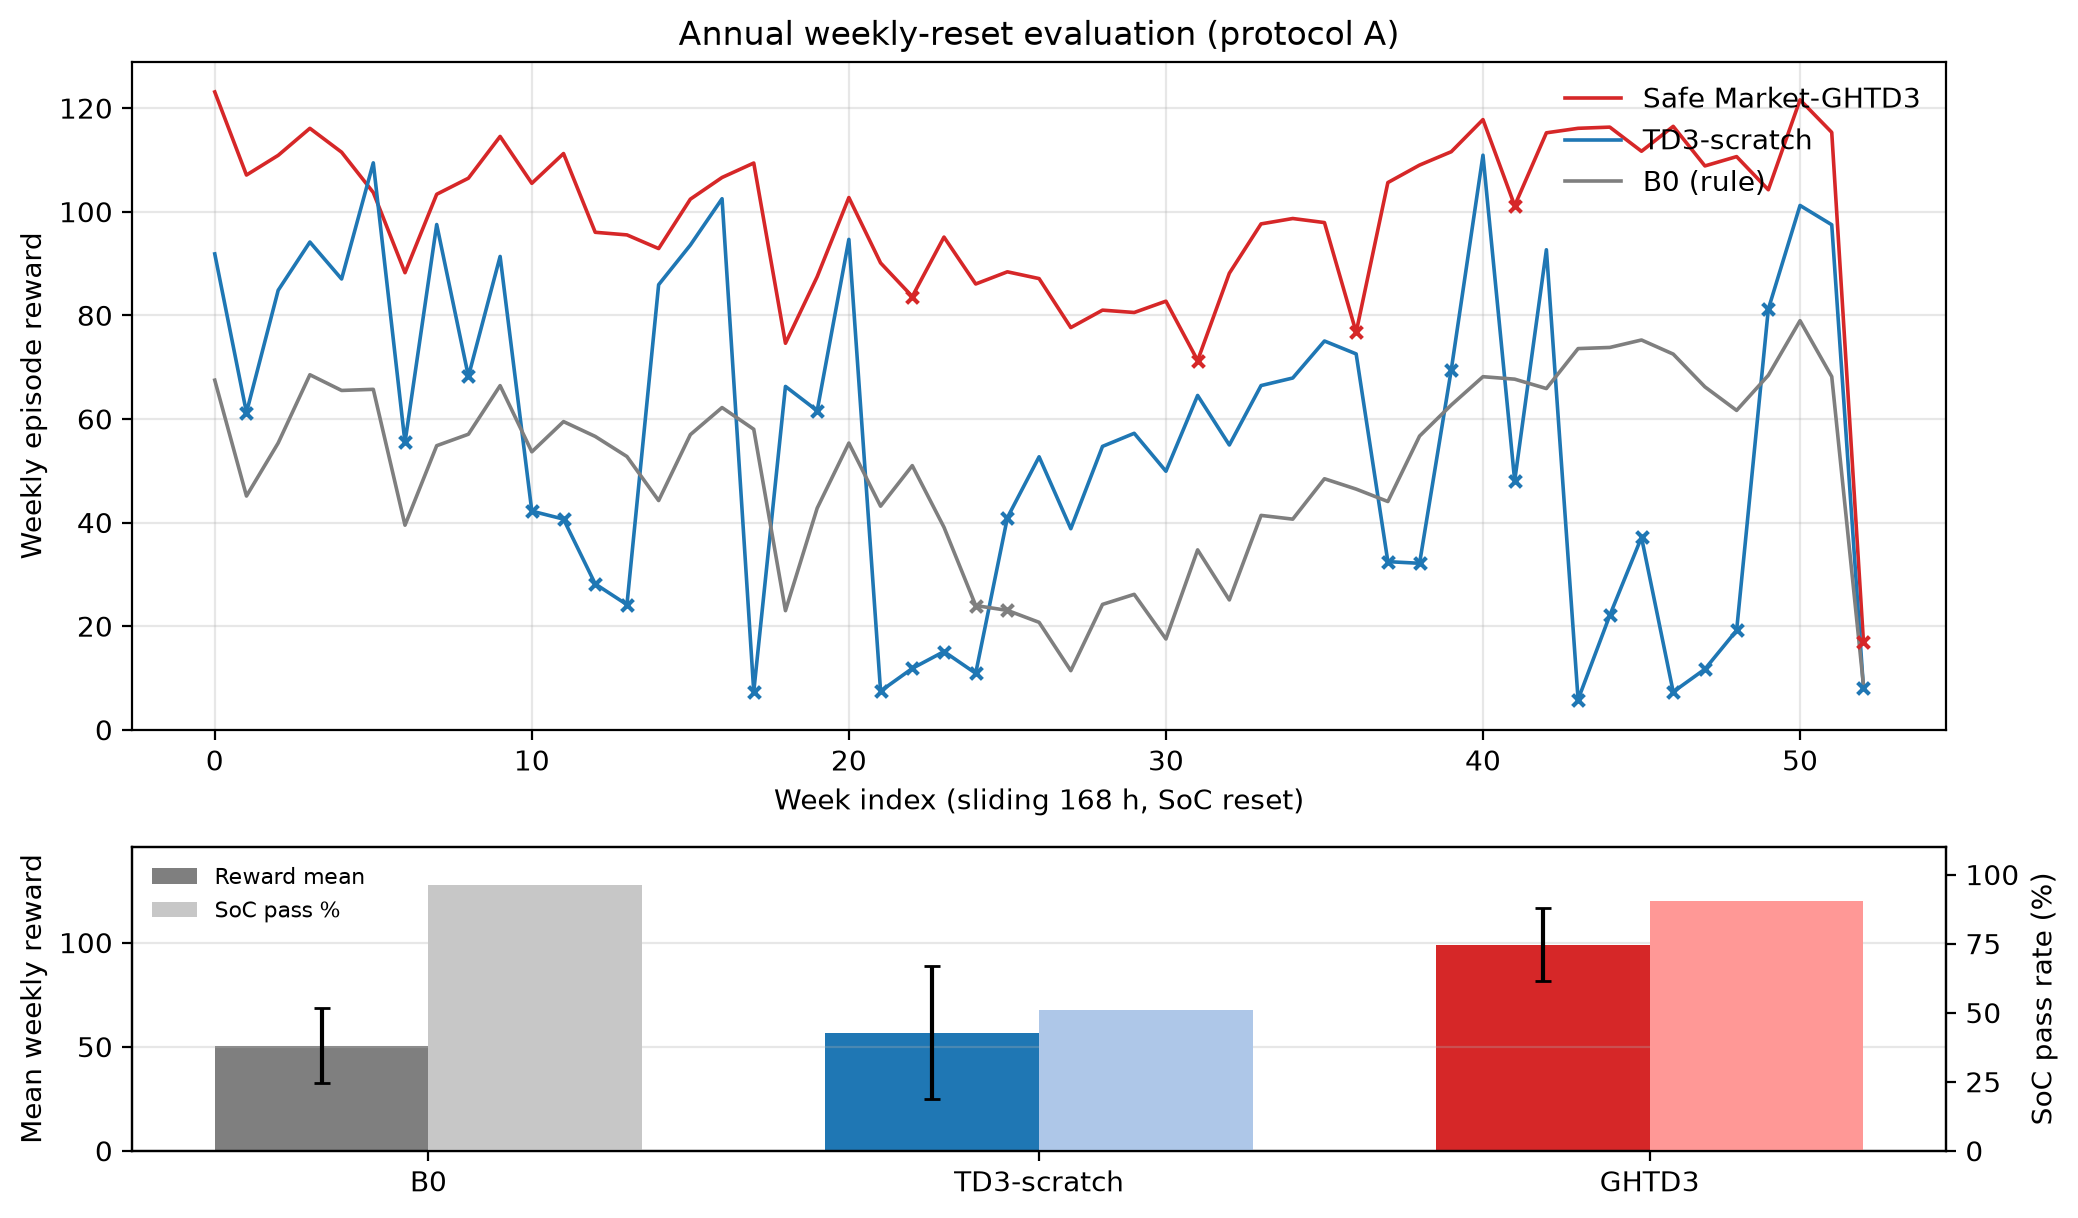
\includegraphics[width=0.9\textwidth]{fig_annual_weekly_reset}
\caption{Weekly-reset annual evaluation (52+ windows) used as a protocol contrast to continuous SoC carry.}
\label{fig:annual-reset}
\end{figure}

\paragraph{Intensity-benchmark carbon.}
The Python economic layer can accumulate an intensity allowance $A_t=\beta E^{\mathrm{th}}_t$ and emissions $E_t=\eta_{\mathrm{th}}E^{\mathrm{th}}_t$, settle $Q=A-E$ at episode end, and expose normalised position, degradation fraction and year progress as three auxiliary observation channels (Figs.~\ref{fig:carbon-pos}--\ref{fig:aux}). Main seasonal tables quote the intensity-benchmark book with $\pi_{\mathrm{CO_2}}=97.49$~CNY/t unless a sensitivity row is marked otherwise.

\begin{figure}[!htbp]
\centering
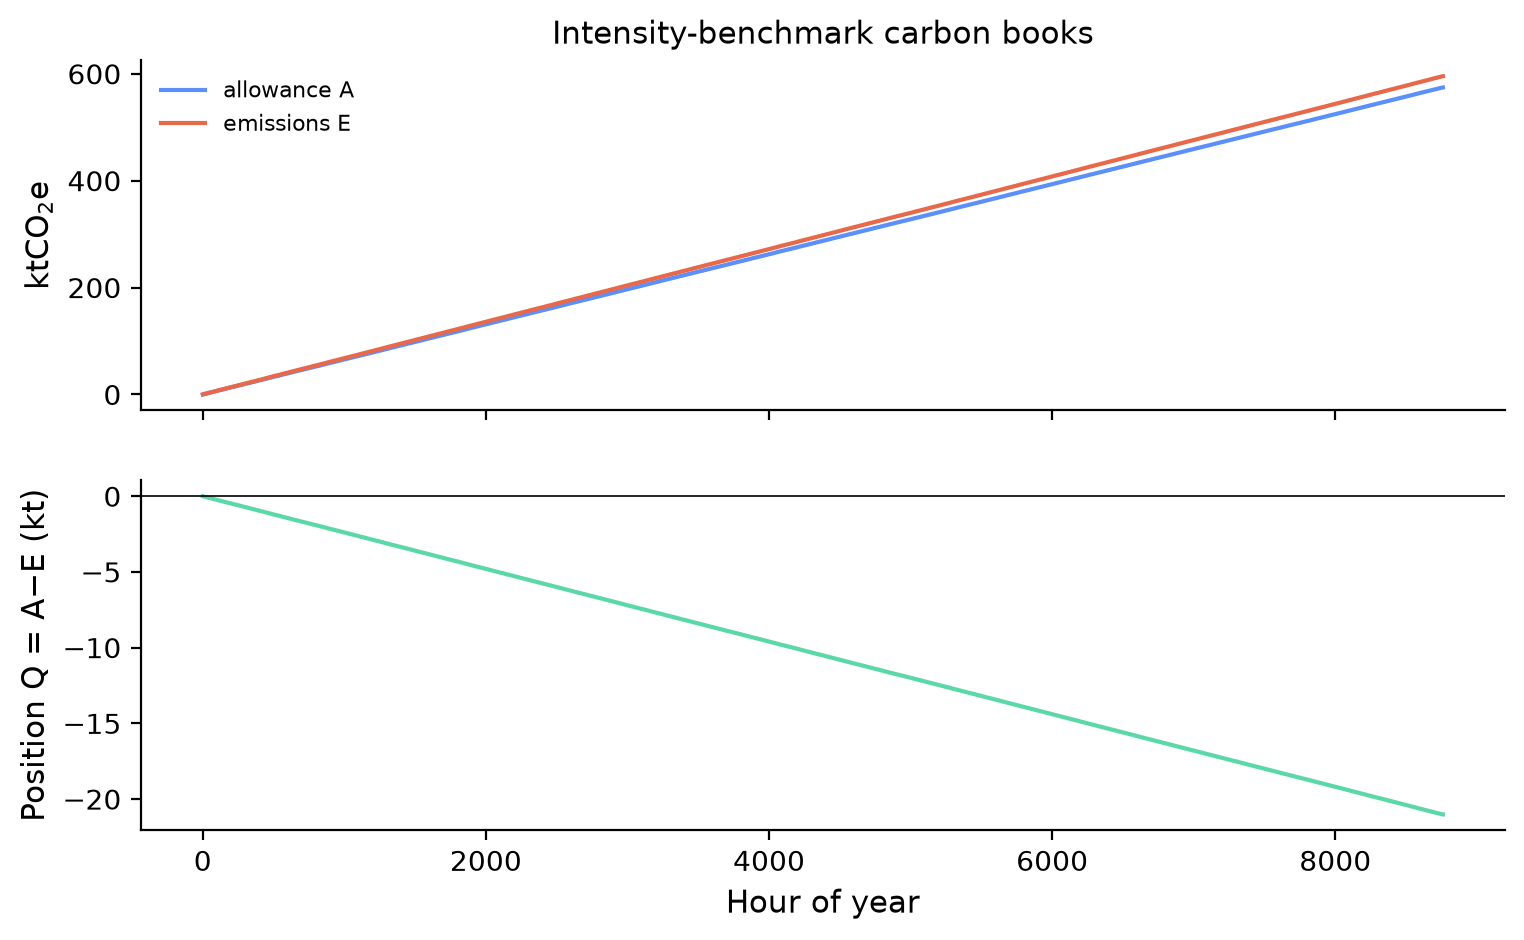
\includegraphics[width=0.92\textwidth]{fig_carbon_position}
\caption{Intensity-benchmark carbon books: cumulative allowance $A$, emissions $E$ and position $Q=A-E$.}
\label{fig:carbon-pos}
\end{figure}

\begin{figure}[!htbp]
\centering
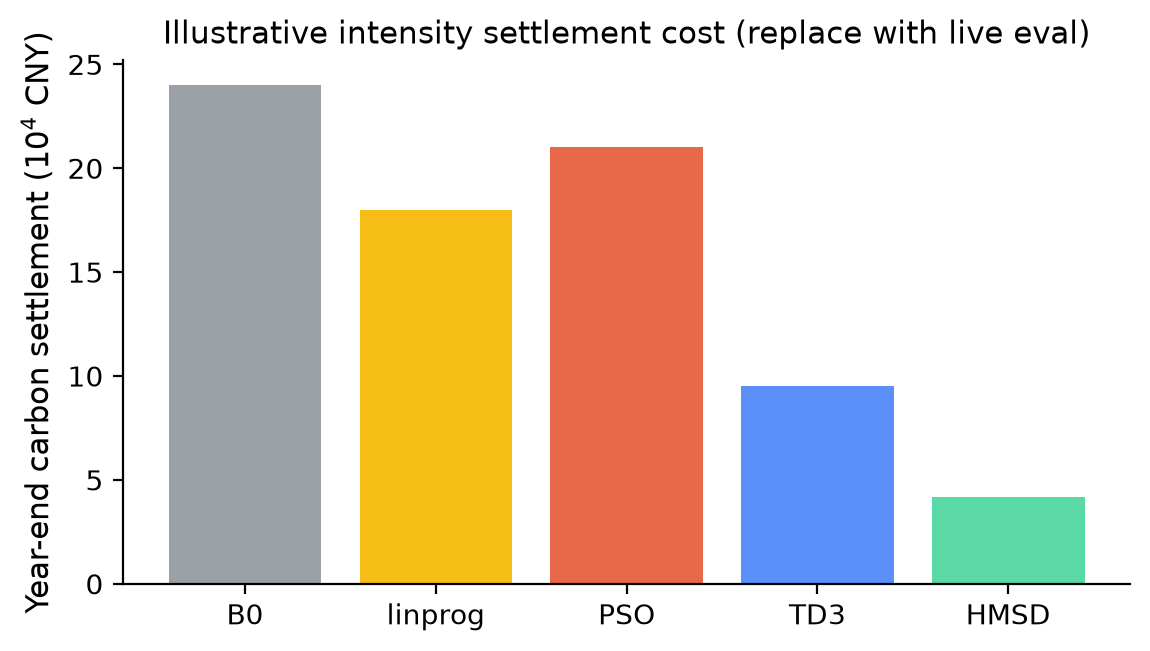
\includegraphics[width=0.78\textwidth]{fig_carbon_settlement}
\caption{Illustrative year-end carbon settlement by method (replace with live continuous-year evals when available).}
\label{fig:carbon-settle}
\end{figure}

\begin{figure}[!htbp]
\centering
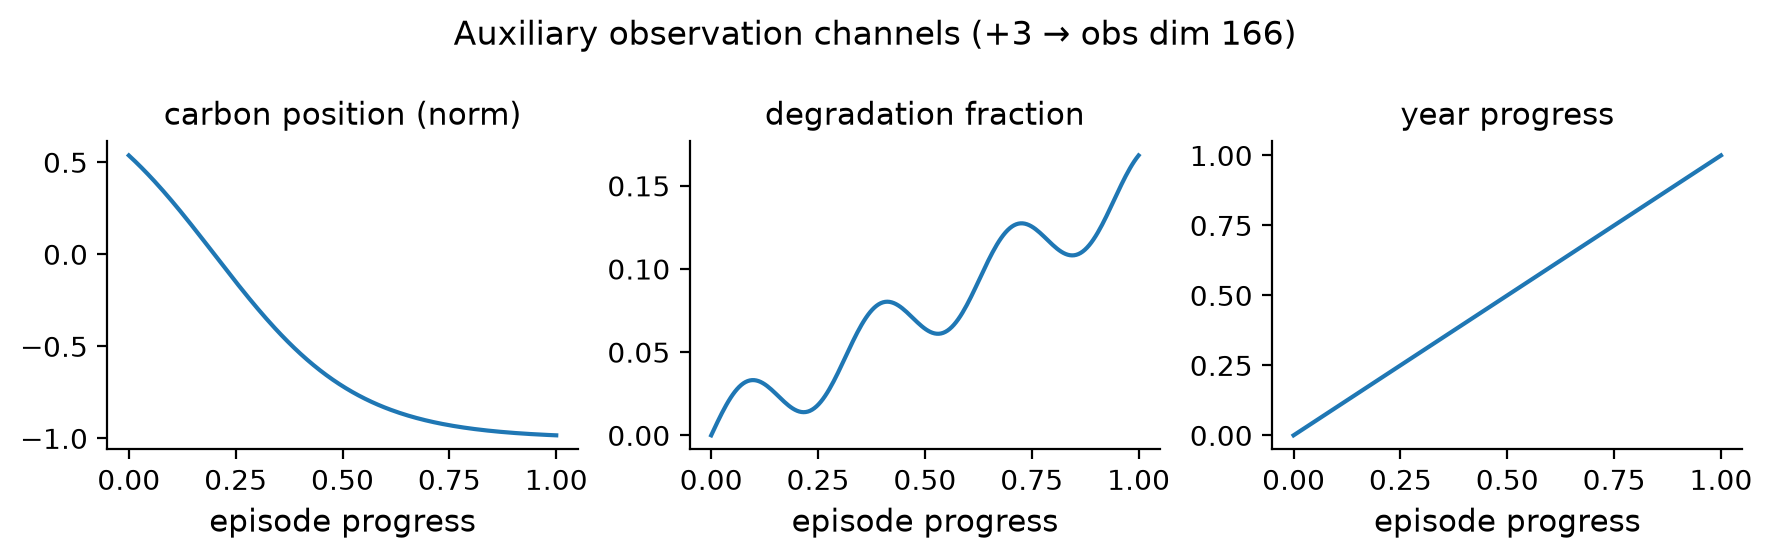
\includegraphics[width=0.92\textwidth]{fig_aux_obs}
\caption{Auxiliary observation channels appended to the physical--forecast--market vector (observation dimension $166$).}
\label{fig:aux}
\end{figure}

\begin{figure}[!htbp]
\centering
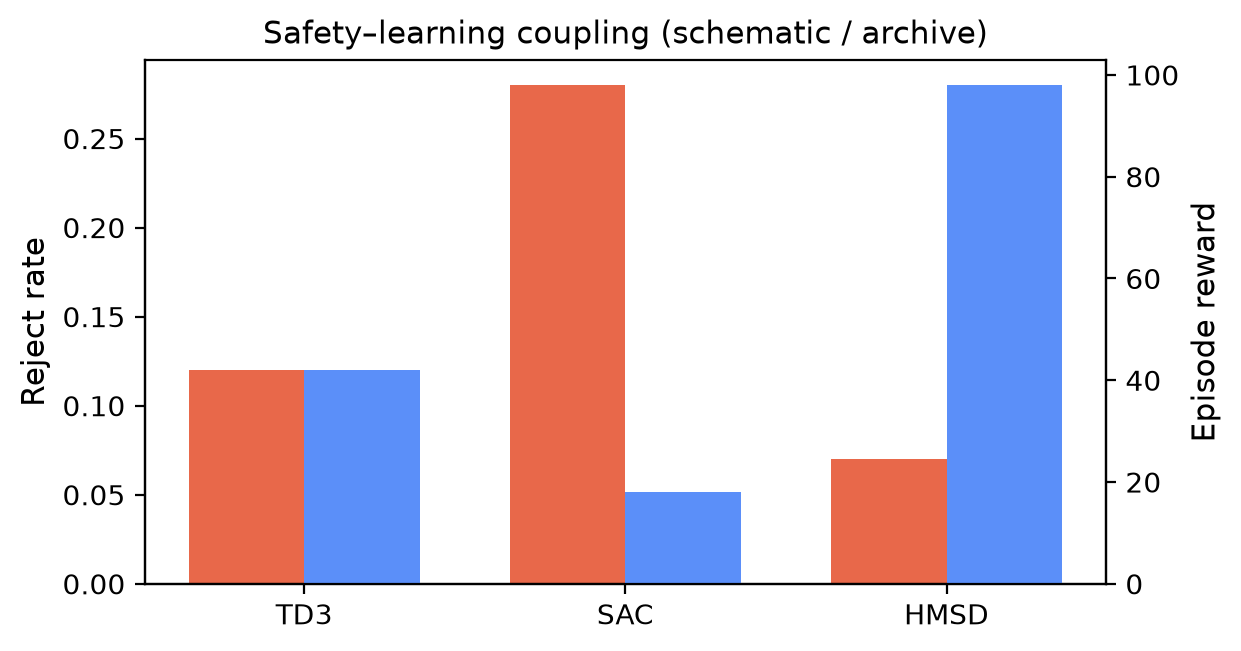
\includegraphics[width=0.78\textwidth]{fig_givesafe_reject}
\caption{Safety--learning coupling: reject rate versus held-out reward across learning agents (archive / schematic).}
\label{fig:reject}
\end{figure}

\bibliographystyle{elsarticle-num}
\bibliography{references}

\end{document}
